\documentclass[10pt, a4paper]{report}
\usepackage{preamble}

\begin{document}

\begin{titlepage}
    \newgeometry{top=4cm, bottom=4cm, left=2cm, right=2cm}
	\centering
    
\includegraphics[width=0.4\linewidth]{epfl.png}\\[0.5cm] 	% University Logo
    \textsc{\LARGE École Polytechnique Fédérale de Lausanne}\\
    [0.7 cm]
    \textsc{\LARGE Master in Computational Sciences and Engineering}\\
    \vspace{\fill}
    \Huge\textbf{\textsc{Rigorous data-driven computation of spectral properties of Koopman operators for dynamical systems}}\\ \vspace{\fill}		
	\textsc{\LARGE Semester Project}\\[0.4cm]
	\rule{\linewidth}{0.2 mm} \\[0.5 cm]
	\begin{minipage}{0.4\textwidth}
    \begin{flushleft} \large
    \emph{Author:}\\
    Ivan \textsc{Bioli} % Your name
    \end{flushleft}
    \end{minipage}
    ~
    \begin{minipage}{0.4\textwidth}
    \begin{flushright} \large
    \emph{Professor:} \\
    Daniel \textsc{Kressner} \\
    \emph{Supervisor:} \\
    Alice \textsc{Cortinovis} \\
    \end{flushright}
    \end{minipage}\\
	[2cm] \Large{June 10, 2022}
	
\end{titlepage}
\restoregeometry

\begin{abstract}
\thispagestyle{empty}
TO DO
\end{abstract}

\clearpage
\thispagestyle{empty}
\tableofcontents

%CONTENT
\pagenumbering{arabic}
\setcounter{page}{1}

\chapter{Introduction}
\lipsum[1-5]

\chapter{Dynamic Mode Decomposition and its variants}
\section{Dynamic Mode Decomposition (DMD)}
Let us go back to the case of a linear dynamical system
\begin{equation*}
    \vb{x}_{n+1} = \vb*{A}\vb{x}_n, \qquad \vb*{A}\in\R^{n\times n}.
\end{equation*}
As already discussed, in order to extract the dynamic characteristics we need to analyze the spectral properties of $\vb{A}$. However, in a data-drive perspective, we cannot assume that we have access to $\vb*{A}$, but only to a sequence of snapshots. Therefore, we are interested in computing the eigenpairs of $\vb{A}$, or at least the dominant ones, from a sequence of snapshots
\begin{equation*}
    \label{krylov_space}
    \vb*{V}_1^N = \left[\vb{v}_1, \vb{v}_2, \dots, \vb{v}_N\right] = \left[\vb{v}_1, \vb*{A}\vb{v}_1, \dots, \vb*{A}^N\vb{v}_1\right].
\end{equation*}
Since the columns of $\vb*{V}_1^N$ span a Krylov subspace, it is natural to apply a Krylov subspace method. As we do not have access to the matrix $\vb*{A}$ and we cannot compute products of vectors by this matrix, we cannot directly apply numerically stable algorithms such as the Arnoldi method, and we can rely only on the sequence of snapshots we are given in input. \emph{Dynamic Mode Decomposition} (DMD) \cite{schmid_dynamic_2010} is a variant of the Arnoldi method that does not require computing multiplications by $\vb*{A}$, nor any knowledge of the matrix. 

Let us first suppose that, after a certain number of iterates, we found an $\vb*{A}$-invariant Krylov subspace and that $\vb{v}_N$ can be expressed as a linear combination of the previous linearly independent snapshots, i.e.
\begin{equation}
    \label{vn_exact}
    \vb{v}_N = a_1 \vb{v}_1 + \dots + a_{N-1} \vb{v}_{N-1} = \vb{V}_1^{N-1}\vb{a}, \qquad \vb{a}\in\R^{N-1}.
\end{equation}
We can rewrite the relation in \eqref{vn_exact} as:
\begin{equation*}
    \vb*{A}\vb*{V}_1^{N-1} = \vb*{V}_2^{N} = \vb*{V}_1^{N-1}\vb*{S}
\end{equation*}
where $\vb*{S}$ is the companion matrix associated with $\vb{a}$, defined by:
\begin{equation}
    \label{S_definition}
    \vb*{S} :=
   \begin{bmatrix}
   0     &        &       &      & a_1 \\
   1     & 0      &       &      & a_2 \\
         & \ddots & \ddots&      & \vdots \\ 
         &        & 1     & 0    & a_{N-2} \\
         &        &       & 1    & a_{N-1} \\
   \end{bmatrix}.
\end{equation}
The eigenvalues of $\vb*{S}$ are also eigenvalues of $\vb*{A}$. Indeed, if $\vb*{S}\vb{x} = \lambda \vb{x}, \,\, \vb{x}\neq 0$ then $\vb{y} = \vb{V}_1^{N-1}\vb{x}\neq 0$ (we assumed that the first $N-1$ snapshots are linearly independent) and $\vb*{A}\vb{y} = \vb*{A}\vb{V}_1^{N-1}\vb{x} = \vb{V}_1^{N-1}\vb*{S}\vb{x} = \lambda \vb{V}_1^{N-1}\vb{x} = \lambda \vb{y}$.

In general, $\vb{v}_N$ does not necessarily belong to the Span of the columns of $\vb*{V}_1^{N-1}$, i.e. in general $\vb*{V}_1^{N}$ is non-singular. However, as $N$ increases the snapshots tend to lie in the same direction (or at least in the same subspace) and we can expect that after a critical number of snapshots $\vb{v}_N$ \emph{almost} lies in the $\Span{(\vb*{V}_1^{N-1})}$, i.e. that the angle between $\vb{v}_N$ and $\Span{(\vb*{V}_1^{N-1})}$ is close to zero. Therefore, again assuming that the previous vectors are linearly independent, we we want to write
\begin{equation}
    \label{vn_error}
    \begin{split}
        & \vb{v}_N = a_1 \vb{v}_1 + \dots + a_{N-1} \vb{v}_{N-1} + \vb{r}, \qquad \text{i.e.}\\
        & \vb*{A}\vb*{V}_1^{N-1}  = \vb*{V}_1^{N-1}\vb*{S} + \vb{r}\vb{e}_{N-1}^T
    \end{split}
\end{equation}
so that we minimize the norm of the residual $\vb{r} = \vb{v}_N - \vb*{V}_1^{N-1}\vb{a}$. To solve the corresponding least square problem, we compute the thin QR-decomposition of $\vb*{V}_1^{N-1} = \vb*{Q}\vb*{R}$ and then we obtain
\begin{equation}
    \label{a_qrleastsquare}
    \vb{a} = \vb*{R}^{-1} \vb*{Q}^*\vb{v}_N = (\vb*{V}_1^{N-1})^{\dagger}\vb{v}_N.
\end{equation}
The eigenvalues $\{\lambda_j\}_{j = 1}^{N-1}$ of the companion matrix $\vb*{S}$ are now approximations of the eigenvalues of $\vb*{A}$ and are called \emph{Ritz values}. The corresponding approximate eigenvectors $\vb{y}_j = \vb*{V}_1^{N-1}\vb{x}_j$, where $\vb{x}_j$ is an eigenvector of $\vb*{S}$ are the so called \emph{Ritz vectors}. The following proposition summarizes the properties of the approximations provided by the above described DMD algorithm.

\begin{prop}[\cite{drmac_data_2017}]
Suppose that $\vb*{V}_1^{N-1}$ is of full column rank and let us define the Krylov subspace $\mathcal{V}_k = \range(V_1^k)$ for $k = 1, \dots, N$. Let $\vb{a}$ be computed solving the least square problem 
\begin{equation*}
    \vb{a} = \argmin_{\vb{x}\in\R^{N-1}}\norm{\vb{v}_N - \vb*{V}_1^{N-1}\vb{x}} = (\vb*{V}_1^{N-1})^{\dagger}\vb{v}_N
\end{equation*}
and let $\vb*{S}$ be the companion matrix associated with $\vb{a}$ as in \eqref{S_definition}. Then:
\begin{enumerate}[label=(\roman*)]
    \item $\vb*{S} = (\vb*{V}_1^{N-1})^{\dagger}\vb*{A}\vb*{V}_1^{N-1} = (\vb*{V}_1^{N-1})^{\dagger}\vb*{V}_2^{N}$ is the matrix representation of the projection onto $\mathcal{V}_{N-1}$ of the linear operator defined by $\vb*{A}$ restricted to $\mathcal{V}_{N-1}$, i.e. $P_{\mathcal{V}_{N-1}}\vb*{A}\rvert_{\mathcal{V}_{N-1}}$, in the Krylov basis $\vb*{V}_1^{N-1}$ of  $\mathcal{V}_{N-1}$.
    \item if $\vb{r} = \vb{v}_N - \vb*{V}_1^{N-1}\vb{a} = 0$ then $\vb*{A}\vb*{V}_1^{N-1}  = \vb*{V}_1^{N-1}\vb*{S}$, and each eigenpair $(\lambda, \vb{x})$ of $\vb*{S}$ yields an eigenpair of $\vb*{A}$, $(\lambda, \vb{y} = \vb*{V}_1^{N-1}\vb{x})$ 
    \item if $\vb{r} = \vb{v}_N - \vb*{V}_1^{N-1}\vb{a} \neq 0$ then $\vb*{A}\vb*{V}_1^{N-1}  = \vb*{V}_1^{N-1}\vb*{S} + \vb{r}\vb{e}_{N-1}^T$ and the residual $\vb{r}$ is orthogonal to $\range(\vb*{V}_1^{N-1})$. Moreover each eigenpair $(\lambda, \vb{x})$ of $\vb*{S}$ yields an approximate eigenpair of $\vb*{A}$, $(\lambda, \vb{y} = \vb*{V}_1^{N-1}\vb{x})$ called Ritz pair.
    \item The Ritz pair is an exact eigenpair of the perturbed matrix 
    \begin{equation}
        \label{delta_def}
        \vb*{A} + \vb*{\Delta A}, \qquad \vb*{\Delta A} = - \vb{r}\vb{e}_{N-1}^T (\vb*{V}_1^{N-1})^{\dagger}
    \end{equation}
    \item if $\vb*{A}$ is diagonalizable with eigenvalues $\lambda_1, \dots, \lambda_d$ and eigenvector matrix $\vb*{M}$, then for each eigenvalue $\lambda$ of $\vb*{S}$ it holds
    \begin{equation*}
    \begin{split}
        \min_{\lambda_i}\abs{\lambda - \lambda_i} &\leq \kappa_2(\vb*{M})\norm{\vb*{\Delta A}}_2 \\
        \min_{\lambda_i}\frac{\abs{\lambda - \lambda_i}}{\abs{\lambda_i}} &\leq \kappa_2(\vb*{M})\norm{\vb*{A}^{-1}\vb*{\Delta A}}_2 \text{if $\vb*{A}$ is non-singular}
    \end{split}
    \end{equation*}
    where $\kappa_2(\vb*{M}) = \norm{\vb*{M}}_2\norm{\vb*{M}^{-1}}_2$ is the condition number in $2$-norm of the matrix $\vb*{M}$.
\end{enumerate} 
\end{prop}
\begin{proof}
Since $\vb*{V}_1^{N-1}$ is of full column rank, then $(\vb*{V}_1^{N-1})^{\dagger} = ((\vb*{V}_1^{N-1})^{*}\vb*{V}_1^{N-1})^{-1}(\vb*{V}_1^{N-1})^{*}$ is the matrix representation of the projection onto $\mathcal{V}_{N-1}$ with input basis the canonical basis and output basis $\vb*{V}_1^{N-1}$. Moreover $\vb*{A}\vb*{V}_1^{N-1} = \vb*{V}_2^{N}$ is the matrix representation of the linear operator defined by $\vb*{A}$ restricted to $\mathcal{V}_{N-1}$, whit input basis $\mathcal{V}_{N-1}$ and output basis the canonical basis. Statement $(i)$ follows by composition.

We have already discussed $(ii)-(iii)$ and we know that $\vb*{A}\vb*{V}_1^{N-1}  = \vb*{V}_1^{N-1}\vb*{S} + \vb{r}\vb{e}_{N-1}^T$. Moreover, since $\vb*{V}_1^{N-1}$ is of full column rank $(\vb*{V}_1^{N-1})^{\dagger}\vb*{V}_1^{N-1} = \vb*{I}_{N-1}$, hence :
\begin{equation*}
    \vb*{V}_1^{N-1}\vb*{S} = \vb*{A}\vb*{V}_1^{N-1} - \vb{r}\vb{e}_{N-1}^T = \vb*{A}\vb*{V}_1^{N-1} - \vb{r}\vb{e}_{N-1}^T (\vb*{V}_1^{N-1})^{\dagger}\vb*{V}_1^{N-1}  = (\vb*{A} + \vb*{\Delta A})\vb*{V}_1^{N-1} 
\end{equation*}
and statement $(iv)$ follows. Finally, applying the Bauer-Fike theorem \cite{golub_matrix_2013} the first bound in $(v)$ follows immediately. For the second bound, observe that if $\vb*{A}$ is non singular we can multiply by $\vb*{A}^{-1}$ the equality $(\vb*{A} + \vb*{\Delta A})\vb{x} = \lambda \vb{x}$, obtaining $(\lambda \vb*{A}^{-1}  - \vb*{A}^{-1}\vb*{\Delta A})\vb{x} = \vb{x}$. Hence from the Bauer-Fike theorem:
\begin{equation*}
    \min_{\lambda_i}\abs{1 - \frac{\lambda}{\lambda_i}} = \min_{\lambda_i}\frac{\abs{\lambda - \lambda_i}}{\abs{\lambda_i}} \leq  \kappa_2(\vb*{M}^{-1})\norm{\vb*{A}^{-1}\vb*{\Delta A}}_2 = \kappa_2(\vb*{M})\norm{\vb*{A}^{-1}\vb*{\Delta A}}_2
\end{equation*}
\end{proof}

\section{SVD-based DMD}
The above mentioned method was the original version of the DMD \cite{schmid_dynamic_2010}. However, even if it mathematically correct and equivalent to the Arnoldi method in exact arithmetic (see \Cref{section_dmd_arnoldi}), an implementation using the companion matrix $\vb*{S}$ gives rise to a numerically unstable algorithm that is usually not capable to extract more than one or two dominant eigenpairs. Indeed, as already pointed out, the matrix $\vb*{V}_1^{N-1}$ might be numerically rank deficient, hence ill conditioned. Therefore, even when a QR-factorization $\vb*{V}_1^{N-1} = \vb*{Q}\vb*{R}$ is available, it is not advised to compute $\vb{a}$ as $\vb{a} = \vb*{R}^{-1}\vb*{Q}\vb{v}_N$ or $\vb*{S}$ as $\vb*{S} = \vb*{R}^{-1}\vb*{Q}\vb*{A}\vb*{V}_1^{N-1}$. 

Using the Singular Value Decomposition (SVD) it is possible to obtain a mathematically equivalent but better-conditioned algorithm, which is particularly useful when $\vb*{V}_1^{N-1}$ is close to singular (it is very likely to happen for large $N$). This second version of the DMD is what nowadays is referred as DMD. Suppose that we computed a SVD of the snapshots matrix
\begin{equation*}
    \vb*{V}_1^{N-1} = \vb*{U}\vb*{\Sigma}\vb*{W}^* \qquad \vb*{\Sigma}\in\R^{N-1\times N-1},
\end{equation*}
we can now rewrite \eqref{vn_error} as
\begin{equation}
    \label{vn_error_rewritten}
    \vb*{A}\vb*{U}\vb*{\Sigma}\vb*{W}^* = \vb*{U}\vb*{\Sigma}\vb*{W}^*\vb*{S} + \vb{r}\vb{e}_{N-1}^T = \vb*{V}_2^N
\end{equation}
and rearranging
\begin{equation}
    \label{S_tilde_definition}
    \vb*{U}^*\vb*{A}\vb*{U} = \vb*{U}^*\vb*{V}_2^N\vb*{W}\vb*{\Sigma}^{-1} =: \widetilde{\vb*{S}}.
\end{equation}
Once we have computed the eigenpairs $\{(\lambda_j, \vb{x}_j)\}_j$ of the matrix $\widetilde{\vb*{S}}$, which in this case is a full matrix and not of companion type, we obtain the Ritz values and vectors as $\{(\lambda_j, \vb*{U}\vb{x}_j)\}_j$. 

Besides the better conditioning, a great advantage of the SVD-based approach over the Arnoldi-based one is the opportunity to account for rank deficiency in $\vb*{V}_1^{N-1}$ and noise in the data by truncating the SVD of $\vb*{V}_1^{N-1}$. Indeed, we might include a first step in which the matrix $\vb*{V}_1^{N-1}$ is approximated by a low-rank matrix with approximately the same \emph{numerical} rank. This is achieved in a standard way, that is truncating the SVD of the matrix $\vb*{V}_1^{N-1}$ as suggested by the Eckhart–Young-Mirsky theorem \cite{golub_matrix_2013}. The use of TSVD can be particularly useful when using data from experiments, as the problem might be ill-conditioned. 

As previously mentioned, the two approaches are equivalent since $\vb*{S}$ and $\widetilde{\vb*{S}}$ are linked through a similarity transformation, as long as $\vb*{V}_1^{N-1}$ is of full column rank and we do not truncate the SVD. This is summarized in the following proposition
\begin{prop}
\label{prop_svd_dmd}
Suppose that $\vb*{V}_1^{N-1}$ is of full column rank and let $\vb*{V}_1^{N-1} = \vb*{U}\vb*{\Sigma}\vb*{W}^{*}$ be its SVD. Given $k\in\{1,2,\dots, N-1\}$, let us define $\vb*{U}_k = \vb*{U}(\,:\,, 1:k)$, $\vb*{W}_k = \vb*{W}(\,:\,, 1:k)$, $\vb*{\Sigma}_k = \vb*{\Sigma}(1:k, 1:k)$ and finally $\widetilde{\vb*{S}} = \vb*{U}_k^*\vb*{V}_2^N\vb*{W}_k\vb*{\Sigma}_k^{-1}$. Then:
\begin{enumerate}[label=(\roman*)]
    \item if $k = N-1$, i.e. if we do not truncate the SVD, then $\widetilde{\vb*{S}}$ is similar to $\vb*{S}$, where $\vb*{S}$ is defined as in \eqref{S_definition} and the similarity is realized by the matrix $\vb*{W}\vb*{\Sigma}^{-1}$.
    \item if $k < N-1$, then $\widetilde{\vb*{S}}$ is the matrix representation in the basis $\vb*{W}_k\vb*{\Sigma}^{-1}_k$ of the projection onto $\range(\vb*{W}_l\vb*{\Sigma}^{-1}_k)$ of the linear operator defined by $\vb*{S}$ restricted to $\range(\vb*{W}_k\vb*{\Sigma}^{-1}_k)$.
    \item $\widetilde{\vb*{S}}$ is the matrix representation in the basis $\vb*{U}_k$ of the projection onto $\range(\vb*{U}_k)$ of the linear operator defined by $\vb*{A}$ restricted to $\range(\vb*{U}_k)$.
\end{enumerate}
\end{prop}
\begin{proof}
Let us first suppose that $k=m$, i.e. that the SVD is not truncated. Then the residual of the least squares solution is orthogonal to the columns of $\vb*{U}$, hence from \eqref{vn_error_rewritten} and \eqref{S_tilde_definition}:
\begin{equation*}
    \begin{split}
    \widetilde{\vb*{S}} & =
    \vb*{U}^*\vb*{V}_2^N\vb*{W}\vb*{\Sigma}^{-1} =
    \vb*{U}^*(\vb*{U}\vb*{\Sigma}\vb*{W}^*\vb*{S} + \vb{r}\vb{e}_{N-1}^T)\vb*{W}\vb*{\Sigma}^{-1} = \\
    & = (\vb*{\Sigma}\vb*{W}^*) \vb*{S} (\vb*{W}\vb*{\Sigma}^{-1}) =
    (\vb*{W}\vb*{\Sigma}^{-1})^{-1} \vb*{S} (\vb*{W}\vb*{\Sigma}^{-1})    
    \end{split}
\end{equation*}
and the matrices $\widetilde{\vb*{S}}$ and $\vb*{S}$ are liked by the stated similarity transformation.

If $k < m$ we can write $\vb*{V}_1^{N-1} ={ \vb*{U}_k\vb*{\Sigma}_k\vb*{W}^{*}_k + \vb*{\delta V}}$, where $\vb*{\delta V} = {\sum_{i = k+1}^{N-1}\sigma_i\vb*{U}(\,:\,, i)\vb*{W}(\,:\,, i)^*}$ is such that $\vb*{U}_k^{*}\vb*{\delta V} = \vb*{\delta V}\vb*{W}_k = \vb*{0}$. Hence we can write \eqref{vn_error} as
\begin{equation*}
    \vb*{A}(\vb*{U}_k\vb*{\Sigma}_k\vb*{W}^{*}_k + \vb*{\delta V}) = (\vb*{U}_k\vb*{\Sigma}_k\vb*{W}^{*}_k + \vb*{\delta V})\vb*{S} + \vb{r}\vb{e}_{N-1}^T = \vb*{V}_2^N
\end{equation*}
Multiplying by $\vb*{U}_k^*$ on the left and by $\vb*{W}_k\vb*{\Sigma}_k^{-1}$ on the right, we get
\begin{equation*}
    \vb*{U}_k^{*}\vb*{A}\vb*{U}_k = (\vb*{W}_k\vb*{\Sigma}^{-1}_k)^{-1} \vb*{S} (\vb*{W}_k\vb*{\Sigma}^{-1}_k) = \widetilde{\vb*{S}} 
\end{equation*}
and the thesis follows.
\end{proof}

The SVD-based version of DMD is summarized in \Cref{alg_dmd}.

\begin{algorithm}
\caption{\textbf{: SVD-based DMD}}
\label{alg_dmd}
\textbf{Input:} $\vb{v}_1,\dots, \vb{v}_N$
\begin{algorithmic}[1]
\State Define the matrices $\vb*{V}_1^{N-1} = \left[\vb{v}_1,\dots,\vb{v}_{N-1}\right]$ and $\vb*{V}_2^{N} = \left[\vb{v}_2,\dots,\vb{v}_{N}\right]$.
\State Compute the (possibly truncated) SVD of $\vb*{V}_1^{N-1} = \vb*{U}\vb*{\Sigma}\vb*{W}^*,\,\, \vb*{\Sigma}\in\R^{p\times p}$.
\State Define the matrix $\widetilde{\vb*{S}} := \vb*{U}^*\vb*{V}_2^N\vb*{W}\vb*{\Sigma}^{-1}$.
\State Compute the eigenpairs $\{(\lambda_j, \vb{x}_j)\}_j$ of $\widetilde{\vb*{S}}$.
\State Compute the Ritz vector corresponding to the Ritz value $\lambda_j$ as $\vb{y}_j = \vb*{U}\vb{x}_j$. 
\end{algorithmic}
\textbf{Output:} Ritz values $\lambda_1,\dots,\lambda_{p}$ and corresponding Ritz vectors $\vb{y}_1,\dots, \vb{y}_p$
\end{algorithm}

\section{DMD and the Arnoldi method}
\label{section_dmd_arnoldi}
The Arnoldi method and the DMD are equivalent in exact arithmetic. In the following section, we will discuss and prove this statement, emphasizing why the Arnoldi algorithm is generally more stable.

The Arnoldi method computes an orthonormal basis of the Krylov subspace spanned by the columns of $\vb*{V}_1^{N-1}$ computing the snapshots implicitly. In particular, if $\vb*{V}_1^{N-1}$ is of full colum rank and therefore the algorithms does not stop, it computes a matrix $\vb*{Q}_{N-1} = \left[\vb{q}_1,\dots, \vb{q}_{N-1}\right]$ with columns that form an orthonormal basis of $\Span{(\vb*{V}_1^{N-1})}$ and: 
\begin{enumerate}[label=(\roman*)]
    \item $\vb*{V}_1^{N-1} = \vb*{Q}_{N-1} \vb*{R}_{N-1}$ is a thin QR-decomposition (with $\vb*{R}_{N-1}$ that is computed implicitly);
    \item $\vb*{H}_{N-1} = \vb*{Q}_{N-1}^* \vb*{A} \vb*{Q}_{N-1}$ is a Hessenberg matrix.
\end{enumerate}
Then the eigenpairs approximations are obtained from the eigenpairs of $\vb*{H}_{N-1}$. This is mathematically equivalent to the DMD algorithm, as specified in the following proposition. 

\begin{prop}
Suppose that $\vb*{V}_1^{N-1}$ is of full column rank. Then the Arnoldi method and the DMD algorithms are equivalent in exact arithmetic, i.e. the Ritz pairs returned by the two algorithms coincide. 
\end{prop}
\begin{proof}
From \eqref{vn_error} and \eqref{a_qrleastsquare} the residual $\vb{r}$ can be written as
\begin{equation*}
    \vb{r} = \vb{v}_N - \vb*{V}_1^{N-1}\vb*{R}_{N-1}^{-1}\vb*{Q}_{N-1}^*\vb{v}_N = \vb{v}_N - \vb*{Q}_{N-1}\vb*{Q}_{N-1}^*\vb{v}_N
\end{equation*}
and therefore $\vb*{Q}_{N-1}^*\vb{r} = \vb*{0}$.Plugging the QR-decomposition into \eqref{vn_error}
\begin{equation*}
    \vb*{A}\vb*{Q}_{N-1}\vb*{R}_{N-1} = \vb*{Q}_{N-1}\vb*{R}_{N-1}\vb*{S} + \vb{r}\vb{e}_{N-1}^T
\end{equation*}
and multiplying by $\vb*{Q}_{N-1}^*$ on the left and by $\vb*{R}_{N-1}^{-1}$ on the right
\begin{equation}
    \label{similarity_arnoldi_dmd}
    \vb*{H}_{N-1} = \vb*{Q}_{N-1}\vb*{A}\vb*{Q}_{N-1} = \vb*{R}_{N-1}\vb*{S}\vb*{R}_{N-1}^{-1}.
\end{equation}
Hence $\vb*{H}_{N-1}$ and $\vb*{S}$ are linked through a similarity transformation and, in particular, have the same eigenvalues. As a consequence of \Cref{prop_svd_dmd}, this is true also if we apply the SVD-based DMD without truncation.

Let $\vb*{M}_{N-1}$ be eigenvector matrix of $\vb*{H}_{N-1}$, then the Ritz vectors returned by the Arnoldi method are the columns of $\vb*{Q}_{N-1}\vb*{M}_{N-1}$. From \eqref{similarity_arnoldi_dmd}, the eigenvector matrix of $\vb*{S}$ is $\vb*{R}_{N-1}^{-1}\vb*{M}_{N-1}$, thus the Ritz vectors returned by the DMD algorithm are the columns of $\vb*{V}_1^{N-1}\vb*{R}_{N-1}^{-1}\vb*{M}_{N-1} = \vb*{Q}_{N-1}\vb*{R}_{N-1}\vb*{R}_{N-1}^{-1}\vb*{M}_{N-1} = \vb*{Q}_{N-1}^{-1}\vb*{M}_{N-1}$ and also the Ritz vectors coincide.
\end{proof}


Although the two algorithms are equivalent mathematically and in exact arithmetic, the Arnoldi algorithm is numerically more stable. Indeed, as the number of snapshots increases, the vectors tend to become linearly dependent and therefore, the matrix $V_1^N$ becomes close to singular, hence ill-conditioned. Even if the problem can be partially solved using the SVD-based DMD and performing a truncated SVD, another major problem is intrinsic to the data-driven approach. One of the major strengths of the Arnoldi algorithm is that it does not even compute the vectors $\vb{x}_j = \vb*{A}^j \vb{x}_0$ because errors are already made in these computations. However, in a data-driven perspective, this is not possible since what we are given is a sequence of snapshots and not the matrix $\vb*{A}$. Hence, we trade-off better stability and convergence properties for an algorithm that only relies on $V_1^N$ and is therefore applicable to snapshots experimentally collected.

To compare numerically the algorithms, we performed 60 iterations with the matrix \texttt{A} of size \texttt{n = 400} defined as \texttt{A = diag(0.95.\^{}(0:n-1))} and random starting vector \texttt{x = rand(n,1)} normalized. \Cref{fig_arnoldi_vs_DMD} shows the convergence of the approximations of the five dominant eigenvalues. It can be seen that the Arnoldi method is able to approximate all of them up to the epsilon-machine-precision. The Arnoldi-based DMD algorithm fails in extracting the second and third dominant eigenvalue, and approximates the first one with an accuracy that is two orders of magnitude lower than the one obtained with the SVD-based DMD. The SVD-based DMD is able to approximate all five dominant eigenvalues, with an accuracy than is lower than the one of the Arnoldi algorithm, but still acceptable. 
\begin{figure}[h]
    \centering
    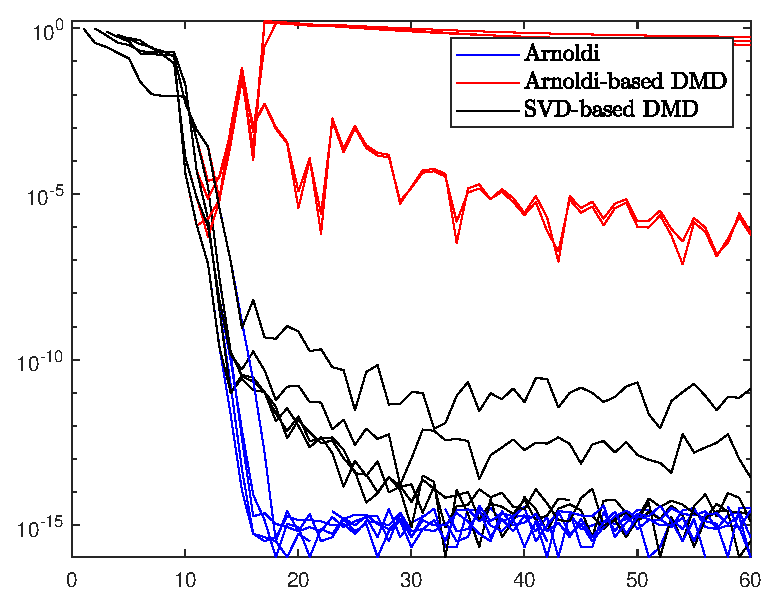
\includegraphics[width=0.5\linewidth]{../code/figures/Arnoldi_vs_DMD.eps}
    \caption{Convergence of the five dominant eigenvalues for the Arnoldi method, the Arnoldi-based DMD algorithm and the SVD-based DMD algorithm. 60 iterations are performed with the matrix \texttt{A} of size \texttt{n = 400} defined as \texttt{A = diag(0.95.\^{}(0:n-1))}.}
    \label{fig_arnoldi_vs_DMD}
\end{figure}

\section{DMD for snapshot data}
The original version of the DMD algorithm \cite{schmid_dynamic_2010} assumes that data consist of a trajectory of snapshots $\vb{v}_1, \dots, \vb{v}_N$ where $\vb{v}_{i+1} = \vb*{A}\vb{v}_{i}$. While this is required to write \Cref{vn_error} with $\vb{S}$ a companion matrix, the SVD-based approach does not exploit this structure. Indeed, as already observed in \cite{tu_dynamic_2014}, \Cref{alg_dmd} can be carried out for general matrices $\vb*{X}_0$ and $\vb*{X}_1$ replacing $\vb*{V}_1^{N-1}$ and $\vb*{V}_2^{N}$ respectively, where we may assume that
\begin{equation}
    \label{dmd_matrices}
    \vb*{X}_0 = \left[\vb{x}_0^{(1)}, \dots, \vb{x}_0^{(M)}\right] \qquad \vb*{X}_1 = \left[\vb{x}_1^{(1)}, \dots, \vb{x}_1^{(M)}\right]
\end{equation}
are such that $\vb{x}_1^{(m)} = \mathbb{A}\vb{x}_0^{(m)}$ for some linear operator $\mathbb{A}$. This allows to generalise DMD to the case of nonlinear dynamics.

Again, let us start with the linear case, and suppose that instead of snapshots along a single trajectory $\vb{v}_1, \vb{v}_2, \dots, \vb{v}_N$ we are given snapshot pairs of the system state, $\{(\vb{x}_0^{(m)}, \vb{x}_1^{(m)})\}_{m = 1}^M$ with $\vb{x}_1^{(m)} = \vb{F}(\vb{x}_0^{(m)}) = \vb*{A}\vb{x}_0^{(m)}$. The first setting is just a particular case of the latter one, with $\vb{x}_0^{(m)} = \vb{v}_m,\,\,\vb{x}_1^{(m)} = \vb{v}_{m+1}$. However, even in the linear case, requiring in input only snapshot pairs instead of one trajectory allows us to explore as many different initial states as we want. This is of particular help if the trajectories tend to converge to an equilibrium. Let us consider $\vb*{X}_0$ and $\vb*{X}_1$ defined as in \eqref{dmd_matrices}, then the best approximation of $A$ that we can get from data is the least-squares solution is $\hat{\vb*{A}} = \vb*{X}_1\vb*{X}_0^{\dagger}$. The eigenvalues of $\vb*{A}$ can now be approximated by the eigenvalues of $\hat{\vb*{A}}$. The DMD eigenvalues and modes are defined as the nonzero eigenvalues and corresponding eigenvectors of $\hat{\vb*{A}}$, respectively.

If the system is nonlinear, then $\hat{\vb*{A}}$ only provides the best-fit linear approximation of $\vb{F}$, but there is no apparent reason why $\vb{F}$ should be well approximated by a linear finite-dimensional operator. However, even if the dynamics is nonlinear the Koopman Operator is linear (but infinite dimensional). Therefore, we could apply the DMD algorithm to observables in order to obtain an approximation of the Koopman eigenvalues and modes. Let us consider a vector-valued observable $\vb{g} = \vb{g}(\vb{x})$ and its measurements over a set of arbitrary initial states $\{\vb{x}_1,\dots, \vb{x}_M\}$ and one step after. Let us define:
\begin{equation}
    \label{dmd_koopman_matrices}
    \begin{split}
        \vb*{G}_0 &= \left[\vb{g}(\vb{x}_1), \dots, \vb{g}(\vb{x}_M)\right] \\
        \vb*{G}_1 &= \left[\vb{g}(\vb{F}(\vb{x}_1)), \dots, \vb{g}(\vb{F}(\vb{x}_M))\right] = \left[\mathcal{K}\vb{g}(\vb{x}_1), \dots, \mathcal{K}\vb{g}(\vb{x}_M)\right].\\
    \end{split}
\end{equation}
In analogy to what has been done in the linear case, $\vb*{K} = \vb*{G}_1\vb*{G}_0^{\dagger}$ provides the best finite-dimensional approximation of the Koopman operator that can be achieved using the available data. Therefore, we can approximate the Koopman eigenvalues and modes from the eigendecomposition of $\vb*{K}$, as summarized in \Cref{alg_koopman_dmd}.

\begin{algorithm}[h]
\caption{\textbf{: DMD for Koopman Operator}}
\label{alg_koopman_dmd}
\textbf{Input:} Measurements of a vector values observable, collected in data matrices $\vb*{G}_0,\,\vb*{G}_1$ defined as in \eqref{dmd_koopman_matrices}.
\begin{algorithmic}[1]
\State Compute the (possibly truncated) SVD of $\vb*{G}_0 = \vb*{U}\vb*{\Sigma}\vb*{W}^*$.
\State Define the matrix $\vb*{K} := \vb*{U}^*\vb*{G}_1\vb*{W}\vb*{\Sigma}^{\dagger}$.
\State Compute the eigenpairs $\{(\lambda_j, \vb{x}_j)\}_j$ of $\vb*{K}$. Each nonzero eigenvalue is a DMD eigenvalue.
\State Compute the modes corresponding to the nonzero eigenvalue $\lambda_j$ as $\vb{v}_j = \vb*{U}\vb{x}_j$. 
\end{algorithmic}
\textbf{Output:} Approximation of the Koopman eigenvalues ($\lambda_j$) and modes ($\vb{v}_j$).
\end{algorithm}


The interpretation of $\vb*{K}$ as the best finite-dimensional approximation of the Koopman Operator gives an idea of why \Cref{alg_koopman_dmd} might work. However, this does not provide a mathematical foundation for the method and indeed in \cite{tu_dynamic_2014, bagheri_koopman-mode_2013} it is argued that in the non-linear case \Cref{alg_koopman_dmd} might not perform well in general. However, under fairly restrictive hypothesis, \Cref{alg_koopman_dmd} outputs approximations of the Koopman modes and associated eigenvalues that from the available data are indistinguishable from the exact ones. We refer the reader to \cite{rowley_spectral_2009, tu_dynamic_2014} for a more precise statement.
\begin{comment}
\textcolor{red}{
\begin{prop}[\cite{rowley_spectral_2009, tu_dynamic_2014}]
Let $\vb{g} = \vb{g}(\vb{x})$ be the vector-valued observable of interest and let $\vb*{G}_0,\, \vb*{G}_1$ be defined as in \eqref{dmd_koopman_matrices}. Let us further assume that
\begin{enumerate}[label=(\roman*)]
    \item each component of $\vb{g}$ lies in the span of the Koopman eigenfunctions;
    \item $\vb*{K}\vb*{G}_0 = \vb*{G}_1$, i.e. the residual of the least-square approximation is zero;
    \item $\vb*{K}$ is diagonalizable.
\end{enumerate}
Then the DMD eigenvalues and modes in output of \Cref{alg_koopman_dmd} are INDISTINGUISHABLE FROM?? Koopman eigenvalues and Koopman eigenmodes. 
\end{prop}}\textcolor{red}{
\begin{proof}
Let $\{(\lambda_j, \vb{v}_j)\}$ be the DMD eigenpair, i.e. $\vb*{K}\vb{v}_j = \lambda_j\vb{v}_j$. Since $\vb*{K}$ is diagonalizable we can write $\vb{g}(\vb{x}_i) = \sum_j c_{ji}\vb{v}_j $ for some coefficients $c_{ji}$. Reading the matrix equality $\vb*{K}\vb*{G}_0 = \vb*{G}_1$ by columns we get:
\begin{equation*}
    \mathcal{K}\vb{g}(\vb{x}_i) = \vb{g}(\vb{F}(\vb{x}_i)) = \vb*{K}\vb{g}(\vb{x}_i) = \sum_j c_{ji}\vb*{K}\vb{v}_j = \sum_j c_{ji}\lambda_j\vb{v}_j.
\end{equation*}
Comparing the previous equation with \eqref{koopman_modes}....
\end{proof}}
\end{comment}

\chapter{Extended Dynamic Mode Decomposition and its variants}
\label{chapter_edmd}
In this third chapter, we introduce Extended Dynamic Mode Decomposition as a method for approximating eigenpairs from a dictionary of observables. In \Cref{section_resdmd} we introduce the problem of spectral pollution, and we explain how Residual DMD (ResDMD) can be used to remove it. Then we present pseudospectra as an effective method to individuate spectral pollution, as well as the use of ResDMD for approximating the pseudospectrum of the Koopman Operator. Finally, in \Cref{section_experiments} we reproduce some of he numerical examples presented in \cite{colbrook_rigorous_2021}.

\section{Extended Dynamic Mode Decomposition (EDMD)}
\label{section_edmd}
The \emph{Extended Dynamic Mode Decomposition} (EDMD), originally presented in \cite{williams_data-driven_2015}, is a method that seeks at approximating the Koopman Operator as a finite dimensional operator and then approximate the Koopman (eigenvalue, eigenfunction, mode) tuples from this finite dimensional approximation. The algorithm requires in input:
\begin{itemize}
    \item a dataset of snapshot pairs of the system state, $\{(\vb{x}_0^{(m)}, \vb{x}_1^{(m)})\}_{m = 1}^M$ with $\vb{x}_1^{(m)} = \vb{F}(\vb{x}_0^{(m)})$;
    \item a dictionary of observables $\mathcal{D} = \{\psi_1, \dots, \psi_K\} \subseteq \mathcal{D}(\mathcal{K})$. Let us define the vector-valued observable $\Psi:\Omega\to\C^{1\times K}$ as $\Psi(x) = [\psi_1(x), \dots, \psi_K(x)]$. The choice of the dictionary $\mathcal{D}$ is not easy and depends on the problem at hand. For the moment, let us assume that $\mathcal{D}$ is rich enough to approximate at least a few of the dominant Koopman eigenfunctions.
\end{itemize}

\subsection{Approximation of $\mathcal{K}$ and its eigenpairs}
Let $\phi\in\Span(\mathcal{D})$, then we can write:
\begin{equation*}
    \phi = \sum_{k=1}^K a_k\psi_k = \Psi\vb{a}, \qquad \vb{a}\in\C^K.
\end{equation*}
We aim at generating $\vb*{K}\in\C^{k\times k}$ finite dimensional approximation of $\mathcal{K}$ such that
\begin{equation}
    \label{k_finite_dimensional}
    \mathcal{K}\vb{\phi} = (\Psi \circ \vb{F})\vb{a} = \Psi\vb*K\vb{a} + r
\end{equation}
where the residual term $r = r(\vb{a}, \vb{x})$ is due to the fact that in general $\Span(\mathcal{D})$ is not $\mathcal{K}$-invariant. To obtain the "best" $\vb*{K}\in\C^{K\times K}$ it is natural to minimize the norm of the point-wise maximum of the residual of all possible $\phi\in\Span(\mathcal{D})$, i.e to solve the following problem \cite{colbrook_rigorous_2021}:
\begin{equation}
    \label{edmd_integral_problem}
    \argmin_{\vb*{K}\in\C^{K\times K}}\int_{\Omega} \max_{\vb{a}\in\C^k \\ \norm{\vb{a}} = 1}\abs{r(\vb{a}, \vb{x})}^2 d\omega(\vb{x}) = 
    \argmin_{\vb*{K}\in\C^{K\times K}}\int_{\Omega} \norm{\Psi(\vb{F}(\vb{x})) - \Psi(\vb{x})\vb*{K}}^2 d\omega(\vb{x}).
\end{equation}

We cannot directly compute the integral, thus we need to use a quadrature rule. We take as quadrature nodes our snapshot data $\{\vb{x}_0^{(m)}\}_{m = 1}^M$ with weights $\{w_m\}_{m = 1}^M$. The discretized problem reads:
\begin{equation}
\label{edmd_discretized_problem}
\begin{split}
    &\argmin_{\vb*{K}\in\C^{k\times k}} \sum_{j=1}^M w_j \norm{\Psi(\vb{F}(\vb{x}_0^{(j)})) - \Psi(\vb{x}_0^{(j)})\vb*{K}}^2 = \\
    = &\argmin_{\vb*{K}\in\C^{k\times k}} \sum_{j=1}^M w_j \norm{\Psi(\vb{x}_1^{(j)}) - \Psi(\vb{x}_0^{(j)})\vb*{K}}^2.
\end{split}    
\end{equation}
If we define the matrices
\begin{align}
\label{w_def}
\vb*{W} = \diag(w_1,\dots,w_M)\in\R_+^{M\times M} \\
\label{psi0_def}
\Psi_0 = \left[\Psi(\vb{x}_0^{(1)})^T,\dots,\Psi(\vb{x}_0^{(M)})^T\right]^T\in\C^{M\times K} \\
\label{psi1_def}
\Psi_1 = \left[\Psi(\vb{x}_1^{(1)})^T,\dots,\Psi(\vb{x}_1^{(M)})^T\right]^T\in\C^{M\times K}
\end{align}
we can write the weighted least-square problem in \eqref{edmd_discretized_problem} as 
\begin{equation}
    \label{edmd_discretized_problem_matrix}
    \argmin_{\vb*{K}\in\C^{k\times k}}\norm{\sqrt{\vb*{W}}(\Psi_1 - \Psi_0\vb*{K})}_F^2.
\end{equation}
The solution of the weighted least squares problem is
\begin{equation}
    \label{discretized_problem_solution}
    (\Psi_0^*\vb*{W}\Psi_0)\vb*{K} = \Psi_0^*\vb*{W}\Psi_1 \,\,\Longrightarrow\,\, \vb*{K} = (\Psi_0^*\vb*{W}\Psi_0)^{\dagger}(\Psi_0^*\vb*{W}\Psi_1),
\end{equation}
where by $\Longrightarrow$ we mean that $\vb*{K}$ is the solution with minimal norm, but to have uniqueness of the solution one might use regularization techniques. If the weights are the same for all quadrature points, then $\vb{K} = (\Psi_0^*\Psi_0)^{\dagger} \Psi_0^*\Psi_1 = \Psi_0^{\dagger}\Psi_1$ and we are back to the transpose of the matrix that we would obtain applying the DMD algorithm with vector-valued observable $\Psi^T$.

Observe that the matrices involved in the computations are
\begin{equation*}
    \label{psi_rewriting}
    \begin{split}
        \Psi_0^*\vb*{W}\Psi_0 & = \sum_{j=1}^M w_j \Psi(\vb{x}_0^{(j)})^* \Psi(\vb{x}_0^{(j)})\\
        \Psi_0^*\vb*{W}\Psi_1 & = \sum_{j=1}^M w_j \Psi(\vb{x}_0^{(j)})^* \Psi(\vb{x}_1^{(j)}).
    \end{split}
\end{equation*}
This rewriting is particularly advantageous when the number of snapshots is much larger than the size of the dictionary, i.e. $M >> K$, because each term of the sum can be computed individually and the products in \eqref{psi_rewriting} can be built iteratively, without the need of explicitly storing the matrices $\Psi_0,\,\Psi_1\in\C^{M\times K}$.

To approximate the eigenvalue-eigenfunction pair of the Koopman Operator, we use the eigenpairs of its finite dimensional approximation $\vb*{K}$. If $\lambda_j$ is an eigenvalue of $\vb*{K}$ with eigenvector $\bm{\xi}_j$, an approximation of an eigenvalue-eigenfunction pair of $\mathcal{K}$ is $(\lambda_j, \phi_j = \Psi\bm{\xi}_j)$.

A few final remarks for practical implementation of EDMD:
\begin{itemize}
    \item by reducing the size of the dictionary, we may assume without loss of generality that the matrix $(\Psi_0^*\vb*{W}\Psi_0)$ is non-singular. However, we might also consider using TSVD when computing its pseudo-inverse in practice.  
    \item Instead of computing the matrix $\vb*{K} = (\Psi_0^*\vb*{W}\Psi_0)^{\dagger}(\Psi_0^*\vb*{W}\Psi_1)$ and then its eigenpairs, it is often numerically more stable to solve the generalized eigenvalue problem $(\Psi_0^*\vb*{W}\Psi_0)\bm{\xi} = \lambda(\Psi_0^*\vb*{W}\Psi_1)\bm{\xi}$.
\end{itemize}

\subsection{Approximation of the Koopman modes for the full state observable}
Let us consider the full state observable
\begin{equation}
    \label{full_state_def}
    \vb{g}(\vb{x}) = 
    \begin{bmatrix}
    g_1(\vb{x}) \\
    \vdots \\
    g_d(\vb{x})
    \end{bmatrix} = 
    \begin{bmatrix}
    \vb{e}_1^*\vb{x} \\
    \vdots \\
    \vb{e}_d^*\vb{x}
    \end{bmatrix} = \vb{x}.
\end{equation}
Let us assume that $g_i\in\Span(\mathcal{D})$ for all $i = 1,\dots,d$. If this is not the case an intermediate step to project $g_i$ onto $\Span(\mathcal{D})$ is required, with the accuracy strongly depending on the choice of the dictionary. If $g_i\in\Span(\mathcal{D})$ we can write
\begin{equation}
    g_i = \sum_{k=1}^K b_{ki}\psi_k = \Psi\vb{b}_i
\end{equation}
and in matrix form
\begin{equation*}
    \vb{g} = \vb*{B}^T\Psi^T = (\Psi\vb*{B})^T, \qquad \vb*{B} = \left[\vb{b}_1, \dots,\vb{b}_d\right]\in\C^{k\times d}.
\end{equation*}
If we choose an orthonormal dictionary this step can be accomplished through the computation of the inner products $b_{ki} = \langle g_i, \psi_k \rangle$. This also accounts for the projection onto $\Span(\mathcal{D})$, if required.

Let $\bm{\Xi} = \left[\bm{\xi}_1,\dots,\bm{\xi}_K\right]$ be the matrix of the eigenvectors of $\vb*{K}$, the vector of approximate Koopman eigenfunctions $\Phi(\vb{x}) = \left[\phi_1(\vb{x}), \dots, \phi_K(\vb{x})\right]$ can be written as $\Phi = \Psi\bm{\Xi}$. Thus
\begin{equation}
    \vb{g} = \vb*{B}^T\Psi^T = \vb*{B}^T(\bm{\Xi}^T)^{-1}\Phi^T = (\bm{\Xi}^{-1}\vb*{B})^T\Phi^T.
\end{equation}
Since $\bm{\Xi}$ is the matrix of the eigenvectors of $\vb*{K}$, its inverse is $\bm{\Xi}^{-1} = \left[\vb{u}_1, \dots, \vb{u}_K\right]$ where $\vb{u}_i$ is the left eigenvector of $\vb*{K}$ also associated with $\lambda_i$ and appropriately scaled so that $\vb{u}_i^*\bm{\xi}_j = \delta_{ij}$. We can therefore compute the left eigenvectors of $\vb*{K}$ and letting  $\vb*{V} = (\vb*{U}^*\vb*{B})^T$, then
\begin{equation}
    \vb{g} = \vb*{V}\Psi^T = \sum_{k=1}^K \vb{v}_k\psi_k,
\end{equation}
i.e. $\vb{v}_j = (\vb{u}_j^*\vb*{B})^T$ is the $j$-th Koopman mode.

In conclusion, as summarized in \Cref{alg_edmd},  once we have computed the finite-dimensional approximation $\vb*{K}$ of the Koopman Operator:
\begin{itemize}
    \item the eigenvalues of $\vb*{K}$ are the EDMD approximation of the Koopman eigenvalues;
    \item the right eigenvectors of $\vb*{K}$ generate the approximation of the eigenfunctions;
    \item the left eigenvectors of $\vb*{K}$ generate the approximation of the Koopman modes.
\end{itemize}
If we are interested in an approximation of only a leading subset of eigenvalues, instead of a complete eigendecomposition of the matrix $\vb*{K}$ Krylov methods or other iterative methods might be considered to efficiently compute only the leading eigenpairs of $\vb*{K}$.

\begin{algorithm}
\caption{\textbf{: Extended Dynamic Mode Decomposition (EDMD)}}
\label{alg_edmd}
\textbf{Input}: Snapshot pairs of the system state, $\{(\vb{x}_0^{(m)}, \vb{x}_1^{(m)})\}_{m = 1}^M$, quadrature weights $\{w_m\}_{m = 1}^M$, dictionary of observables $\mathcal{D} = \{\psi_1, \dots, \psi_K\} \subseteq \mathcal{D}(\mathcal{K})$
\begin{algorithmic}[1]
\State Define the matrices $\vb*{W}$ \eqref{w_def}, $\Psi_0$ \eqref{psi0_def}, $\Psi_1$ \eqref{psi1_def}. 
\State Compute the matrices $(\Psi_0^*\vb*{W}\Psi_0)$ and $(\Psi_0^*\vb*{W}\Psi_1)$ .
\State Solve the generalized eigenvalue problem $(\Psi_0^*\vb*{W}\Psi_0)\bm{\xi} = \lambda(\Psi_0^*\vb*{W}\Psi_1)\bm{\xi}$.
\State Obtain the eigenfunctions as $\Phi = \Psi\bm{\Xi}$.
\If{want to compute eigenmodes}
    \State Write the (projection onto $\Span(\mathcal{D})$ of the) full observable $\vb{g}$ as $\vb{g} = \vb*{B}^T\Psi^T$.
    \State Compute the left eigenvectors $\vb{u}_j$ of $\vb*{K} = (\Psi_0^*\vb*{W}\Psi_0)^{\dagger}(\Psi_0^*\vb*{W}\Psi_1)$.
    \State Compute $\vb*{V} = (\vb*{U}^*\vb*{B})^T$, i.e $\vb{v}_j = (\vb{u}_j^*\vb*{B})^T$.
\EndIf
\end{algorithmic}
\textbf{Output:} Approximation of the Koopman eigenvalues ($\lambda_j$), eigenfunctions ($\phi_j$) and, possibly, eigemodes ($\vb{v}_j$).
\end{algorithm}


\section{Spectral pollution and Residual DMD (ResDMD)}
\label{section_resdmd}
To compute the eigenvalues of the Koopman Operator, we approximate the infinite-dimensional operator $\mathcal{K}$ by a finite matrix. Therefore, even if some of the eigenvalues produced by the EDMD algorithm are reliable, most of them are not. \emph{Pseudospectra} \cite{trefethen_spectra_2005} are a tool that allow us to detect this so called \emph{spectral pollution} \cite{colbrook_rigorous_2021}, i.e. spurious eigenvalues of the matrix $\vb*{K}$ that are only due to the discretization and have no connection with the latent Koopman Operator.

\begin{definition}[Pseudospectrum of a square matrix]
Given a matrix $\vb*{A}\in\C^{n\times n}$ and $\varepsilon > 0$, the $\varepsilon$-pseudospectrum of $\vb*{A}$ is defined as
\begin{equation}
    \label{pseudospectrum_matrix_def}
    \sigma_{\varepsilon}(\vb*{A}) = \left\{ \lambda\in\C \text{ : } \norm{(\vb*{A} - \lambda \vb*{I})^{-1}}_2 \geq \frac{1}{\varepsilon}\right\} = \left\{ \lambda\in\C \text{ : } \sigma_{\mathrm{min}}(\vb*{A} - \lambda \vb*{I}) \leq \varepsilon \right\} %\bigcup_{\norm{\vb*{B}} \leq \varepsilon} \sigma(\vb*{A}+ \vb*{B}),
\end{equation}
where $\sigma_{\mathrm{min}}(\vb*{M})$ indicates the minimum singular value of the matrix $\vb*{M}$.
\end{definition}
In analogy with the second form of previous definition, we can define the pseudospectrum of a rectangular matrix pencil as follows.
\begin{definition}[Pseudospectrum of a rectangular matrix pencil]
Given two rectangular matrices $\vb*{A},\vb*{B} \in\C^{m\times n}$ and $\varepsilon > 0$, the $\varepsilon$-pseudospectrum of the matrix pencil $\vb*{A}- \lambda \vb*{B}$ is defined as
\begin{equation}
    \label{pseudospectrum_matrix_pencil_def}
    \sigma_{\varepsilon}(\vb*{A}, \vb*{B}) = \left\{ \lambda\in\C \text{ : } \sigma_{\mathrm{min}}(\vb*{A} - \lambda \vb*{B}) \leq \varepsilon \right\} %\bigcup_{\norm{\vb*{B}} \leq \varepsilon} \sigma(\vb*{A}+ \vb*{B}),
\end{equation}
The pseudospectrum of a rectangular matrix $\vb*{A}\in\C^{m\times n}$ is defined as $    \sigma_{\varepsilon}(\vb*{A}, \vb*{I})$ where
\begin{equation}
    \vb*{I} = \begin{bmatrix} \vb*{I}_n \\ \vb*{0}_{m-n,n}\end{bmatrix} \text{ if $n<m$}, \qquad \vb*{I} = \begin{bmatrix} \vb*{I}_m & \vb*{0}_{m,n-m}\end{bmatrix} \text{ if $m<n$}.
\end{equation}
\end{definition}
However, $\mathcal{K}$ is an infinite dimensional operator and might be unbounded, hence following \cite{colbrook_rigorous_2021} we can define
\begin{equation}
    \label{pseudospectrum_koopman_def}
    \sigma_{\varepsilon}(\mathcal{K}) = \mathrm{cl}\left( \left\{ \lambda\in\C \text{ : } \norm{(\mathcal{K} - \lambda \cdot \mathrm{id})^{-1}} \geq \frac{1}{\varepsilon}\right\} \right) = \mathrm{cl}\left( \bigcup_{\norm{\vb*{B}} \leq \varepsilon} \sigma(\mathcal{K}+ \vb*{B}) \right)
\end{equation}
where $\mathrm{id}$ is the identity operator and $\mathrm{cl}$ is the closure of a set.



\subsection{ResDMD to remove spectral pollution}
The \emph{Residual DMD} (ResDMD) algorithm performs the same steps of EDMD, but then discards the approximate eigenpairs $\{(\lambda_j,\, \phi_j)\}_j$ that have a residual above a certain prescribed tolerance $\varepsilon$. Given a candidate eigenpair $(\lambda, \phi)$ of $\mathcal{K}$, where $\phi = \Psi\bm{\xi}$, to measure its accuracy we can consider the relative residual
\begin{equation}
    \label{residual_definiton}
    \begin{split}
        &\mathrm{res}(\lambda, \phi)^2 = \frac{\int_{\Omega} \abs{[\mathcal{K}\phi](x) - \lambda\phi(x)}^2\,\,d\omega(x)}{\int_{\Omega} \abs{\phi(x)}^2\,\,d\omega(x)} 
        = \frac{\langle (\mathcal{K} - \lambda \cdot\mathrm{id})\phi, (\mathcal{K} - \lambda \cdot \mathrm{id})\phi \rangle}{\langle\phi , \phi \rangle} = \\
        & = \frac{\sum_{j,k = 1}^K \overline{\xi}_j\xi_k \left( \langle\mathcal{K}\psi_k, \mathcal{K}\psi_j\rangle - \lambda \langle\psi_k, \mathcal{K}\psi_j\rangle - \overline{\lambda}\langle\mathcal{K}\psi_k, \psi_j\rangle + \abs{\lambda}^2 \langle\psi_k, \psi_j\rangle\right)}{\sum_{j,k = 1}^K \overline{\xi}_j\xi_k \langle\psi_k, \psi_j\rangle}.
    \end{split}
\end{equation}
Once again, this integral cannot be computed exactly and to approximate it we use the same quadrature rule used to approximate \eqref{edmd_integral_problem}. Hence:
\begin{equation}
    \label{residual_approx}
    \begin{split}
        \mathrm{res}(\lambda, \phi)^2 &\approx \frac{\sum_{j,k = 1}^K \overline{\xi}_j\xi_k \left( (\Psi_1^*\vb*{W}\Psi_1)_{jk} - \lambda (\Psi_1^*\vb*{W}\Psi_0)_{jk} - \overline{\lambda}(\Psi_0^*\vb*{W}\Psi_1)_{jk} + \abs{\lambda}^2 (\Psi_0^*\vb*{W}\Psi_0)_{jk}\right)}{\sum_{j,k = 1}^K \overline{\xi}_j\xi_k (\Psi_0^*\vb*{W}\Psi_0)_{jk}} = \\ 
        & = \frac{\bm{\xi}^* \left((\Psi_1^*\vb*{W}\Psi_1) - \lambda (\Psi_1^*\vb*{W}\Psi_0) - \overline{\lambda}(\Psi_0^*\vb*{W}\Psi_1) + \abs{\lambda}^2 (\Psi_0^*\vb*{W}\Psi_0)\right) \bm{\xi}}{\bm{\xi}^*(\Psi_0^*\vb*{W}\Psi_0)\bm{\xi}} =: \widetilde{\mathrm{res}}^2(\lambda, \phi).
    \end{split}
\end{equation}
If $\widetilde{\mathrm{res}}(\lambda, \phi) > \varepsilon$, the eigenpair $(\lambda, \phi)$ is discarded. This algorithm is summarized in \Cref{alg_resdmd}. Observe that to compute the approximation of the residual we only need to compute $(\Psi_1^*\vb*{W}\Psi_1)$, because the other matrices are already computed in the standard EDMD algorithm. 

\begin{algorithm}
\caption{\textbf{: Residual Dynamic Mode Decomposition (ResDMD)}}
\label{alg_resdmd}
\textbf{Input}: Snapshot pairs of the system state, $\{(\vb{x}_0^{(m)}, \vb{x}_1^{(m)})\}_{m = 1}^M$, quadrature weights $\{w_m\}_{m = 1}^M$, dictionary of observables $\mathcal{D} = \{\psi_1, \dots, \psi_K\} \subseteq \mathcal{D}(\mathcal{K})$, tolerance $\varepsilon > 0$.
\begin{algorithmic}[1]
\State Execute \Cref{alg_edmd}.
\State Compute the matrix $(\Psi_1^*\vb*{W}\Psi_1)$.
\For{each approximate eigenpair $(\lambda_j,\phi_j)$}
    \State Compute $\widetilde{\mathrm{res}}(\lambda_j, \phi)_j$ as in \eqref{residual_approx}.
    \If {$\widetilde{\mathrm{res}}(\lambda_j, \phi)_j \geq \varepsilon$}
        \State Discard the approximate eigenpair $(\lambda_j,\phi_j)$.
    \EndIf
\EndFor
\end{algorithmic}
\textbf{Output:} Approximation of the eigenvalues ($\lambda_j$), eigenfunctions ($\phi_j$) with $\widetilde{\mathrm{res}}(\lambda_j, \phi)_j < \varepsilon$
\end{algorithm}

The above-described cleanup procedure avoids spectral pollution and if the quadrature converges, in the large data limit, removes eigenpairs with a residual above the prescribed tolerance $\varepsilon$ and retains only eigenpairs that are inside the $\varepsilon$-pseudospectrum of $\mathcal{K}$. This is precised in the following proposition.
\begin{prop}[\cite{colbrook_rigorous_2021}, Theorem 4.1]
Assume that the quadrature rule converges, i.e. that
\begin{equation*}
    \lim_{M\to+\infty}(\Psi_0^*\vb*{W}\Psi_0)_{jk} = \langle \psi_j, \psi_k \rangle, \quad
    \lim_{M\to+\infty}(\Psi_0^*\vb*{W}\Psi_1)_{jk} = \langle \psi_j, \mathcal{K}\psi_k \rangle, \quad
    \lim_{M\to+\infty}(\Psi_1^*\vb*{W}\Psi_1)_{jk} = \langle \mathcal{K}\psi_j, \mathcal{K}\psi_k \rangle.
\end{equation*}
Let us denote by $\Lambda$ the eigenvalues in the output of \Cref{alg_resdmd}, then
\begin{equation}
    \limsup_{M\to+\infty} \max_{\lambda\in\Lambda}\norm{(\mathcal{K} - \lambda)^{-1}}^{-1} \leq \epsilon.
\end{equation}
\end{prop}

\subsection{ResDMD to approximate the pseudospectrum}
In spite of the fact that the eigenvalues returned by \Cref{alg_resdmd} lie in the $\varepsilon$-pseudospectrum (in the large data limit), the eigenvalues of $\vb*{K}$ might not approximate the whole spectrum of $\mathcal{K}$ and therefore it might not be possible to approximate the whole $\varepsilon$-pseudospectrum of $\mathcal{K}$ using \Cref{alg_resdmd}. A simple modification of \Cref{alg_resdmd} allows us to draw an approximation of the $\varepsilon$-pseudospectrum of $\mathcal{K}$ starting from a grid of points in the complex plane. Given a point $z_j\in\C$ on a grid, we search the function $\psi_j$ in $\Span(\mathcal{D})$ that minimizes $\mathrm{res}(z_j, \phi)$, i.e. we solve
\begin{equation}
    \label{grid_continuous}
    \tau_j = \min_{\vb{g}\in\C^K} \mathrm{res}(z_j, \Psi\vb{g}), \qquad \vb{g}_j = \argmin_{\vb{g}\in\C^K} \mathrm{res}(z_j, \Psi\vb{g}).
\end{equation}
Following \eqref{residual_approx}, the discretized problem reads:
\begin{equation}
    \label{grid_discretized}
    \tau_j = \min_{\vb{g}\in\C^K} \frac{\vb{g}^*\vb*{D}(z_j)\vb{g}}{\vb{g}^*(\Psi_0^*\vb*{W}\Psi_0)\vb{g}}\,\,, \qquad \vb{g}_j = \argmin_{\vb{g}\in\C^K} \frac{\vb{g}^*\vb*{D}(z_j)\vb{g}}{\vb{g}^*(\Psi_0^*\vb*{W}\Psi_0)\vb{g}}
\end{equation}
\begin{equation}
    \label{D(z)_definition}
    \begin{split}
        \vb*{D}(z_j) &= (\Psi_1^*\vb*{W}\Psi_1) - z_j (\Psi_1^*\vb*{W}\Psi_0) - \overline{z}_j(\Psi_0^*\vb*{W}\Psi_1) + \abs{z_j}^2 (\Psi_0^*\vb*{W}\Psi_0) =\\ 
        & = (\Psi_1 - z_j\Psi_0)^*\vb*{W}(\Psi_1 - z_j\Psi_0).
    \end{split}
\end{equation}
The matrices $(\Psi_0^*\vb*{W}\Psi_0)$ and $\vb*{D}(z_j)$ are hermitian positive semidefinite. If we also assume that $\Psi_0$ has full column rank, from the properties of the Rayleigh quotient solving \eqref{grid_discretized} is equivalent to finding the smallest eigenvalue and the associated eigenvector of the generalized eigenvalue problem $\vb*{D}(z_j)\vb{g} = \tau(\Psi_0^*\vb*{W}\Psi_0)\vb{g}$, which allows for a more efficient computation. This algorithm, proposed in \cite{colbrook_rigorous_2021}, is summarized in \Cref{alg_pseudospectrum}. Convergence guarantees for the approximation of the $\varepsilon$-pseudospectrum can be found in \cite{colbrook_rigorous_2021}.

\begin{algorithm}
\caption{\textbf{: ResDMD for pseudospectrum approximation}}
\label{alg_pseudospectrum}
\textbf{Input}: Snapshot pairs of the system state, $\{(\vb{x}_0^{(m)}, \vb{x}_1^{(m)})\}_{m = 1}^M$, quadrature weights $\{w_m\}_{m = 1}^M$, dictionary of observables $\mathcal{D} = \{\psi_1, \dots, \psi_K\} \subseteq \mathcal{D}(\mathcal{K})$, tolerance $\varepsilon > 0$, grid $z_1, \dots, z_k \in\C$.
\begin{algorithmic}[1]
\State Define the matrices $\vb*{W}$ \eqref{w_def}, $\Psi_0$ \eqref{psi0_def}, $\Psi_1$ \eqref{psi1_def}. 
\State Compute the matrices $(\Psi_0^*\vb*{W}\Psi_0)$, $(\Psi_0^*\vb*{W}\Psi_1)$ and $(\Psi_1^*\vb*{W}\Psi_1)$.
\For{each $z_j$ in the grid}
\State Solve $\tau_j = \min_{\vb{g}\in\C^K} \mathrm{res}(z_j, \Psi\vb{g}),\,\, \vb{g}_j = \argmin_{\vb{g}\in\C^K} \mathrm{res}(z_j, \Psi\vb{g})$.
\EndFor
\end{algorithmic}
\textbf{Output:} Estimate of the $\varepsilon$-pseudospectrum $\{z_j\,:\,\tau_j < \varepsilon\}$ and corresponding approximate eigenfunctions $\{\vb{g}_j\,:\,\tau_j < \varepsilon\}$. 
\end{algorithm}

The following proposition allows to rewrite the pseudospectrum approximation provided by \Cref{alg_pseudospectrum} as the pseudospectrum either of a rectangular matrix pencil or of a rectangular matrix.
\begin{prop}
\label{prop_pseudospectrum}
Let us assume that $\Psi_0$ has full column rank and let us consider the singular value decomposition $\sqrt{\vb*{W}}\Psi_0 = \vb*{U}\bm{\Sigma}\vb*{V}$, where $\vb*{U}\in\C^{M\times K}$ and $\bm{\Sigma},\vb*{V}\in\C^{K\times K}$. Then the approximation of the pseudospectrum of the Koopman operator provided by \Cref{alg_pseudospectrum} coincides with the pseudospectrum of the rectangular matrix pencil
\begin{equation}
    \sqrt{\vb*{W}}\Psi_1 \vb*{V}\bm{\Sigma}^{-1} - \lambda\vb*{U}.
\end{equation}
Moreover if the columns of $\vb*{U}_{\perp}$ complete the columns of $\vb*{U}$ to an orthonormal basis of $\C^{M}$, then the pseudospectrum approximation coincides also with the pseudospectrum of the rectangular matrix
\begin{equation}
    \begin{bmatrix}
    \vb*{U}^*\sqrt{\vb*{W}}\Psi_1 \vb*{V}\bm{\Sigma}^{-1}\\
    \vb*{U}_{\perp}^*\sqrt{\vb*{W}}\Psi_1 \vb*{V}\bm{\Sigma}^{-1}
    \end{bmatrix} = 
    \begin{bmatrix}
    \bm{\Sigma}\vb{V}^*(\Psi_0^\dagger \Psi_1)\vb{V}\bm{\Sigma}^{-1}\\
    \vb*{U}_{\perp}^*\sqrt{\vb*{W}}\Psi_1 \vb*{V}\bm{\Sigma}^{-1}
    \end{bmatrix}.
\end{equation}
\end{prop}
\begin{proof}
Let $z\in\C$ and let us consider the corresponding residual:
\begin{equation*}
\begin{split}
    \tau(z) &= \min_{\vb{g}\in\C^K} \frac{\vb{g}^*\vb*{D}(z)\vb{g}}{\vb{g}^*(\Psi_0^*\vb*{W}\Psi_0)\vb{g}} = \min_{\vb{g}\in\C^K} \frac{\vb{g}^*\vb*{D}(z)\vb{g}}{\vb{g}^*(\vb*{V}\bm{\Sigma}\vb*{V}^*)^2\vb{g}} =  \min_{\vb{v}\in\C^K} \frac{\vb{v}^*(\vb*{V}\bm{\Sigma}^{-1}\vb*{V}^*)\vb*{D}(z)(\vb*{V}\bm{\Sigma}^{-1}\vb*{V}^*)\vb{v}}{\vb{v}^*\vb{v}} = \\
    &= \lambda_{\min}\left((\vb*{V}\bm{\Sigma}^{-1}\vb*{V}^*)\vb*{D}(z)(\vb*{V}\bm{\Sigma}^{-1}\vb*{V}^*)\right) = \lambda_{\min}\left(\vb*{C}(z)^*\vb*{C}(z)\right) = \sigma_{\min}(\vb*{C}(z))^2
\end{split}
\end{equation*}
where from \eqref{D(z)_definition} we can write $\vb*{C}(z) = \sqrt{\vb*{W}}(\Psi_1 - z\Psi_0)\vb*{V}\bm{\Sigma}^{-1}\vb*{V}^*$. Hence $\tau(z) = \sigma_{\min}(\vb*{C}(z))^2 \leq \varepsilon^2$ if and only if $\sigma_{\min}(\vb*{C}(z)) \leq \varepsilon$. Now observe that
\begin{equation*}
    \begin{split}
        \sigma_{\min}(\vb*{C}(z)) &= \sigma_{\min}(\sqrt{\vb*{W}}(\Psi_1 - z\Psi_0)\vb*{V}\bm{\Sigma}^{-1}\vb*{V}^*) = \sigma_{\min}(\sqrt{\vb*{W}}(\Psi_1 - z\vb*{U}\bm{\Sigma}\vb*{V}^*)\vb*{V}\bm{\Sigma}^{-1}\vb*{V}^*) = \\
        &= \sigma_{\min}(\sqrt{\vb*{W}}(\Psi_1 - z\vb*{U}\bm{\Sigma}\vb*{V}^*)\vb*{V}\bm{\Sigma}^{-1}) = \sigma_{\min}(\sqrt{\vb*{W}}\Psi_1\vb*{V}\bm{\Sigma}^{-1} - z\vb*{U})
    \end{split}
\end{equation*}
from which follows the first statement. 

Moreover $\vb*{Q} = [\vb*{U}\,\lvert\,\vb*{U}_\perp]$ is an unitary matrix, hence multiplying by $Q$ on the left the singular values are preserved, yielding:
\begin{equation*}
    \begin{split}
        \sigma_{\min}(\vb*{C}(z)) &= \sigma_{\min}(\vb*{Q}^*\sqrt{\vb*{W}}\Psi_1\vb*{V}\bm{\Sigma}^{-1} - z\vb*{Q}^*\vb*{U}) = \\
        & = \sigma_{\min}\left( 
        \begin{bmatrix}
        \vb*{U}^*\sqrt{\vb*{W}}\Psi_1 \vb*{V}\bm{\Sigma}^{-1}\\
        \vb*{U}_{\perp}^*\sqrt{\vb*{W}}\Psi_1 \vb*{V}\bm{\Sigma}^{-1}
        \end{bmatrix} - z 
        \begin{bmatrix}
        \vb*{I}_K\\
        \vb*{0}_{M-K, K}\\
        \end{bmatrix}
        \right).
    \end{split}
\end{equation*}
Finally one can write the upper part of the matrix as:
\begin{equation*}
    \vb*{U}^*\sqrt{\vb*{W}}\Psi_1 \vb*{V}\bm{\Sigma}^{-1} = \bm{\Sigma} \vb*{V}^* \vb*{V}\bm{\Sigma}^{-1}\vb*{U}^*\sqrt{\vb*{W}}\Psi_1 \vb*{V}\bm{\Sigma}^{-1} = \bm{\Sigma}\vb{V}^*(\Psi_0^\dagger \Psi_1)\vb{V}\bm{\Sigma}^{-1}.
\end{equation*}
\end{proof}

From the previous rewriting, one can use standard techniques for the computation of pseudospectra of rectangular matrices \cite{wright_pseudospectra_2002}, as long as $M$ is not too big. Observe indeed that the matrix pencil in \Cref{prop_pseudospectrum} is of size $M\times K$, while the generalized eigenvalue problems in \Cref{alg_pseudospectrum} involve matrices of size $K\times K$.

\section{Numerical Examples}
\label{section_experiments}
In this section we reproduce two numerical examples from Section 4 of \cite{colbrook_rigorous_2021}.

\subsection{Gauss iterated map}
\label{sect_gauss_iterated_map}
The Gauss iterated map is a function $F:\R\to\R$ defined by $F(x) =\exp(\alpha x^2) + \beta $, where $\alpha$ and $\beta$ are parameters. We consider the case $\alpha = 2$ and $\beta = 1-\exp(-\alpha) = 1 - e^{-2}$, with state space $\Omega = [-1, 0]$ and the Lebesgue measure. Observe that with such a choice of the parameters, $F$ maps $\Omega$ onto itself, as necessary to have a well defined dynamical system on $\Omega$. As a dictionary of observable $\mathcal{D}$ we consider the first $K$ normalized Legendre polynomials transplanted to the interval $\Omega$. To understand the influence on the accuracy of the algorithm of the choice of the snapshot pairs $\{(\vb{x}_0^{(m)}, \vb{x}_1^{(m)})\}_{m = 1}^M$, which are the nodes of the quadrature rule, we consider four different types of quadrature rule:
\begin{itemize}
    \item Gauss-Legendre: $\{\vb{x}_0^{(m)}\}_{m = 1}^M$ are the Gauss-Legendre quadrature nodes transplanted to the interval $\Omega$, with $\{w_m\}_{m = 1}^M$ the corresponding quadrature weights.
    \item Trapezoidal: $\vb{x}_0^{(m)} = -1 + \frac{m-1}{M-1}$, with $w_m = \frac{1}{M-1},\,\,m = 2,\dots, M-1$ and $w_1 = w_M = \frac{1}{2(M-1)}$.
    \item Riemann sum: $\vb{x}_0^{(m)} = -1 + \frac{m-1}{M-1}$, with $w_m = \frac{1}{M-1},\,\,m = 1,\dots, M$.
    \item Montecarlo: $\{\vb{x}_0^{(m)}\}_{m = 1}^M$ are chosen uniformly at random in over the interval $\Omega$, with $w_m = \frac{1}{M-1},\,\,m = 1,\dots, M$. 
\end{itemize}

\Cref{fig_resdmd_quadrature_comparison} shows the approximations of the eigenvalues of the Koopman Operator computed using DMD, EDMD and ResDMD for each of the four quadrature rules. \Cref{gauss_pseudospectrum_convergence} shows the approximation of the $\varepsilon$-pseudospectrum for $\varepsilon = 0.3,\,0.1,\,0.01,\,0.001$ computed using \Cref{alg_pseudospectrum} and the convergence of the different quadrature rules measured as $\max_{1\leq j,k \leq K} \abs{(\Psi_0^* W \Psi_1)_{jk} - \langle\mathcal{K}\psi_k, \psi_j\rangle}$.

It can be seen that for the Montecarlo and the Riemann Sums quadrature rules, which use the same weights for all quadrature points, EDMD and DMD compute the same eigenvalues (magenta dots and green pluses overlap in \Cref{fig_resdmd_quadrature_comparison}). The outputs of the two algorithms are slightly dissimilar for the Trapezoidal rule, which changes the weights only at the extremes, while they significantly differ for the Gauss-Legendre rule.

The convergence rates are in agreement with standard theoretical results on numerical integration \cite{quarteroni_numerical_2007}, with the Gauss-Legendre quadrature converging exponentially and the other quadrature rules polynomially. It can be understood that if one has the possibility of choosing the initial condition of the snapshot data, selecting them wisely can make the discretized problem significantly closer to the continuous one. This has a strong impact also on the accuracy of the eigenvalues computed using \Cref{alg_resdmd}. Indeed, the more accurate is the computation of the residual's integral, the more eigenvalues can be removed due to a too high residual, as shown in \Cref{fig_resdmd_quadrature_comparison}.

\begin{figure}[h]
\centering
\makebox[\textwidth][c]{
    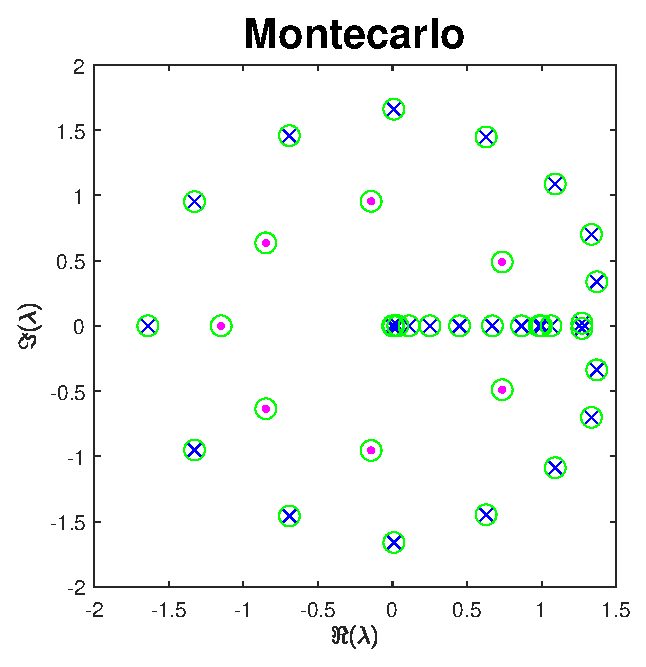
\includegraphics[width=0.25\linewidth]{../code/figures/gauss_map/ResDMD_Montecarlo.eps}
    \hspace*{\fill}
    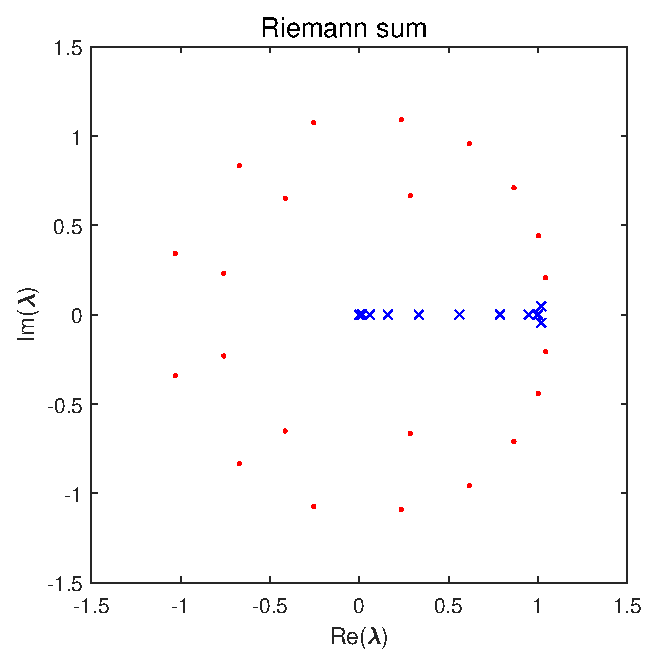
\includegraphics[width=0.25\linewidth]{../code/figures/gauss_map/ResDMD_Riemann.eps}
    \hspace*{\fill}
    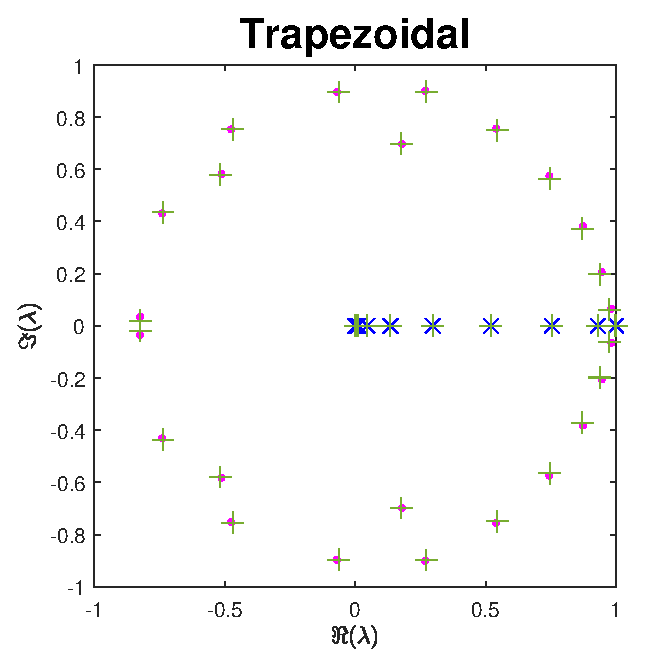
\includegraphics[width=0.25\linewidth]{../code/figures/gauss_map/ResDMD_Trapezoidal.eps}
    \hspace*{\fill}
    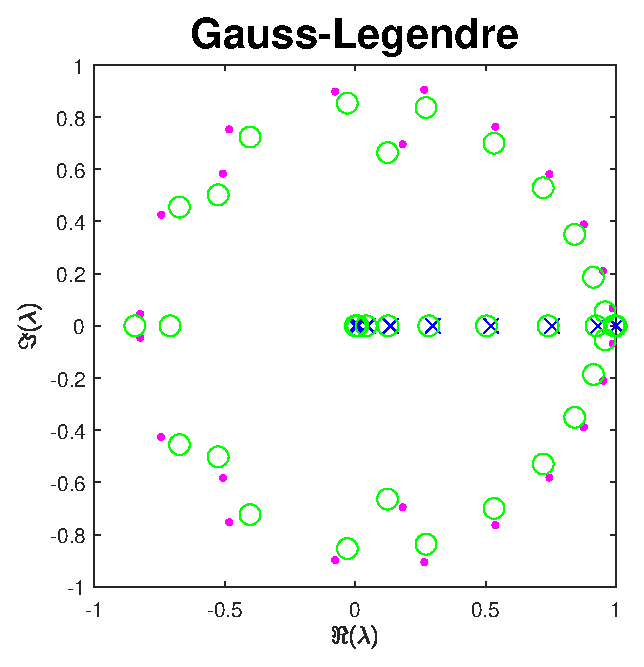
\includegraphics[width=0.25\linewidth]{../code/figures/gauss_map/ResDMD_Gauss-Legendre.eps}
    \hspace*{\fill}
}
\caption{Approximations of the eigenvalues of the Koopman Operator associated with the Gauss iterated map computed with the DMD algorithm (green circles) and the EDMD algorithm (magenta dots and blue crosses), using different quadrature rules. The approximate eigenvalues are computed using $K=40$ observables and $M = 100$ quadrature points. The blue crosses indicate the eigenvalues retained by ResDMD, with tolerance $\varepsilon = 0.01$.}
\label{fig_resdmd_quadrature_comparison}
\end{figure}

\begin{figure}[h]
\makebox[\textwidth][c]{
    \begin{subfigure}{0.45\textwidth}
        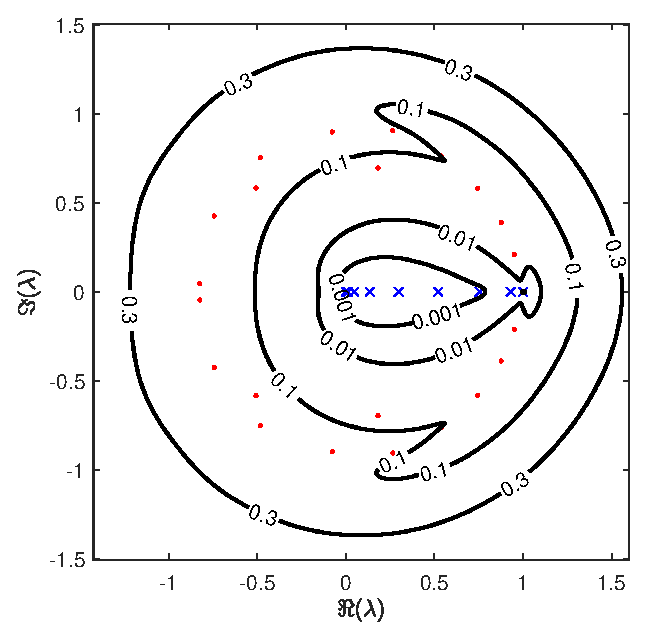
\includegraphics[width=\linewidth]{../code/figures/gauss_map/pseudospectra_contour.eps}
        \caption{Pseudospectral contours}
        \label{gauss_contours}
    \end{subfigure}\hspace*{\fill}
    \begin{subfigure}{0.45\textwidth}
        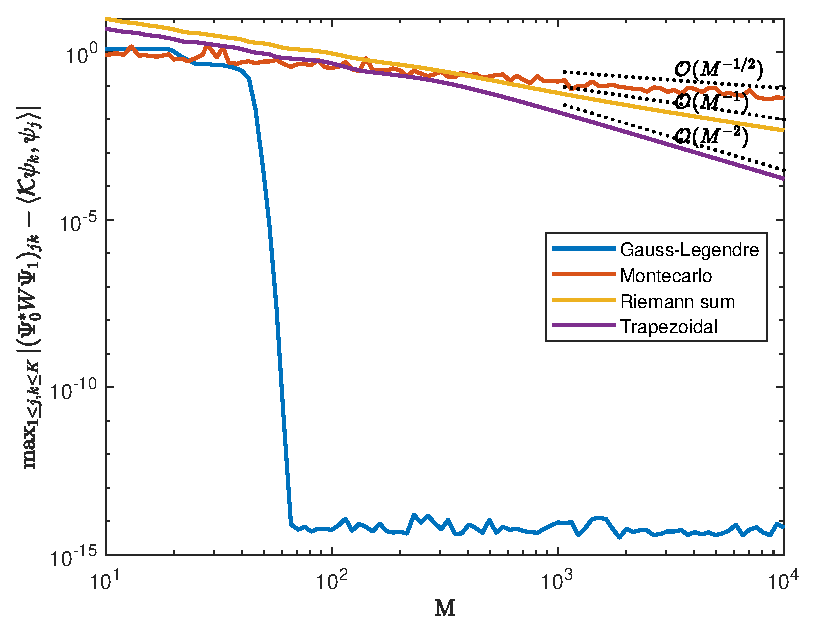
\includegraphics[width=\linewidth]{../code/figures/gauss_map/Galerkin_convergence.eps}
        \caption{Convergence of the quadrature rules}
        \label{gauss_convergence}
    \end{subfigure}\hspace*{\fill}
    }
    \caption{Contour lines of the $\varepsilon$-pseudospectrum for $\varepsilon = 0.3,\,0.1,\,0.01,\,0.001$ computed using \Cref{alg_pseudospectrum} with dictionary of $K=40$ observables (\Cref{gauss_contours}) and convergence of one of the approximate integrals for the different quadrature rules measured as $\max_{1\leq j,k \leq K} \abs{(\Psi_0^* W \Psi_1)_{jk} - \langle\mathcal{K}\psi_k, \psi_j\rangle}$ (\Cref{gauss_convergence}).}
    \label{gauss_pseudospectrum_convergence}
\end{figure}

\subsection{Nonlinear pendulum}
Let us consider the continous-time dynamical system of the nonlinear pendulum. The state variable is $\vb{x} = (x_1, x_2) = (\theta, \dot{\theta}) \in \Omega = [-\pi, \pi]_{\text{per}} \times \R$ and the differential equation governing the motion is
\begin{equation}
    \label{pendulum_equation}
    \dot{\vb{x}} = 
    \begin{bmatrix}
    \dot{x}_1 \\
    \dot{x}_2
    \end{bmatrix} = 
    \begin{bmatrix}
    x_2 \\
    -\sin(x_1)
    \end{bmatrix}.
\end{equation}
We consider the corresponding discrete-time dynamical system with time-step $\Delta_t = 0.5$ and the associated Koopman Operator. The system is Hamiltonian and hence the Koopman Operator is unitary \cite{koopman_hamiltonian_1931}.

The choice of the dictionary of observables is now more complex, because the function governing the motion is vector-valued (with two components) and periodic in the first component. Since the motion is periodic in $x_1\in[-\pi,\pi]_{\text{per}}$, it is natural to use the Fourier basis $\{e_n\}_{n\in\mathbb{Z}}$ in $x_1$ to describe the motion in this direction. Similarly, to approximate the motion in the direction of $x_2$ one might decide to use the Hermite functions $\{h_n\}_{n\in\mathbb{N}}$, which form a basis of the Hilbert space $L^2(\R)$. Therefore, we would ideally consider observables of the form $\phi(x_1, x_2) = \sum_{n\in\mathbb{Z},\,m\in\mathbb{N}} \alpha_{n,m} e_n(x_1)\cdot h_m(x_2)$ for some coefficients $\{\alpha_{n,m}\}\in\C$. However, our dictionary of observables must be finite and we need to decide a criterion to truncate the sum. Observe that there isn't a natural ordering as if the indices were in $\mathbb{N}$ or $\mathbb{Z}$. Since we want to be able to approximate the (components of the) full state observable, it is important to have the indices $\{(n,0)\}_{n=0}^{n_{\max}}$ and $\{(0,m)\}_{m=-m_{\max}}^{m_{\max}}$ with $n_{\max},\,m_{\max}$ as high as possible. Selecting the indices in the rectangle $\{(n,m)\,:\,-n_{\max}\leq n\leq n_{\max},\,\, 0\leq m\leq m_{\max}\}$ would make the size of the dictionary grow too fast in $n_{\max}$ and $m_{\max}$, thus we use an hyperbolic cross approximation \cite{dung_hyperbolic_2017}, i.e. we select the indices in the hyperbolic cross $\{(n,m)\,:\, \max(n,1)\cdot \max(m,1)\leq N \}$, where $N$ is called the order of the hyperbolic cross approximation.

Using \Cref{alg_pseudospectrum} we compute an approximation of the $\varepsilon$-pseudospectrum for $\varepsilon = 0.25$, first using $K=193$ observables and $M = 10^4$ data points, then employing $K=1265$ and $M = 9 \times 10^4$. As the size $K$ of the dictionary increases, the approximation of the $\varepsilon$-pseudospectrum approaches the annulus with internal radius 0.75 and external radius 1.25(see \Cref{pendulum_pseudospectrum}). We also compute approximation of the eigenfunctions associated with the eigenvalues $\lambda = \exp(0.4932 i), \,\lambda = \exp(0.9765 i), \,\lambda = \exp(1.4452 i), \,\lambda = \exp(1.8951 i), \,$ (see \Cref{pendulum_phase_portraits}).

\begin{figure}[h]
\makebox[\textwidth][c]{
    \begin{subfigure}{0.45\textwidth}
        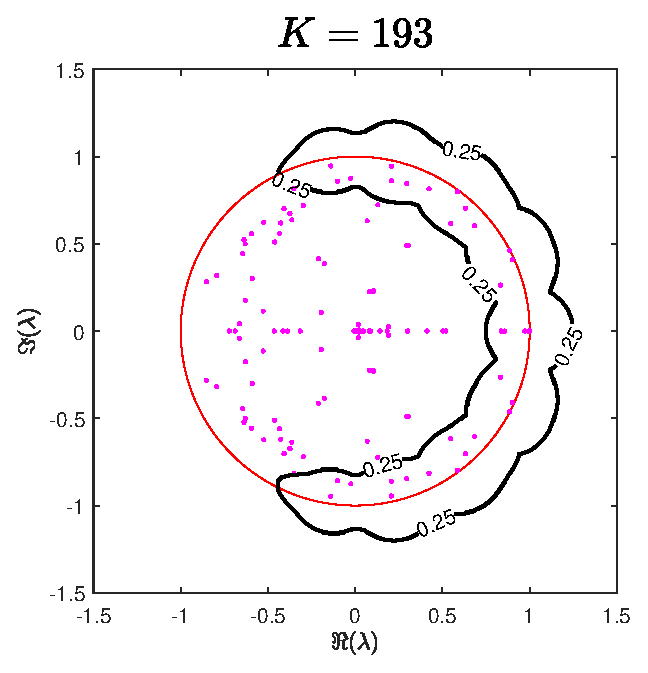
\includegraphics[width=\linewidth]{../code/figures/pendulum/pendulum_N193.eps}
    \end{subfigure}\hspace*{\fill}
    \begin{subfigure}{0.45\textwidth}
        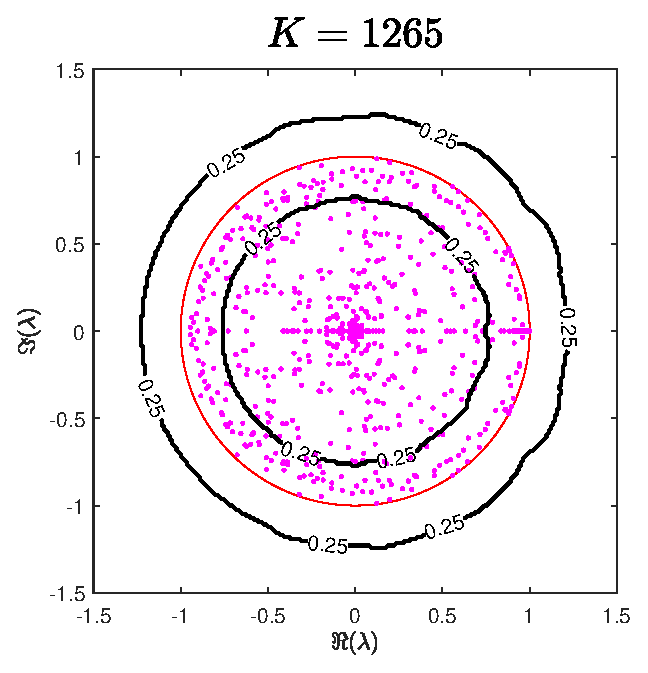
\includegraphics[width=\linewidth]{../code/figures/pendulum/pendulum_N1265.eps}
    \end{subfigure}\hspace*{\fill}
        }
    \caption{Contour lines of the $\varepsilon$-pseudospectrum for $\varepsilon = 0.25$ computed using \Cref{alg_pseudospectrum} with hyperbolic cross approximation. On the left the approximation obtained using a dictionary of $K=193$ observables and $M = 10^4$ data points, on the right the one obtained with $K=1265$ and $M = 9 \times 10^4$.}
    \label{pendulum_pseudospectrum}
\end{figure}

\begin{figure}[h]
\centering
\makebox[\textwidth][c]{
        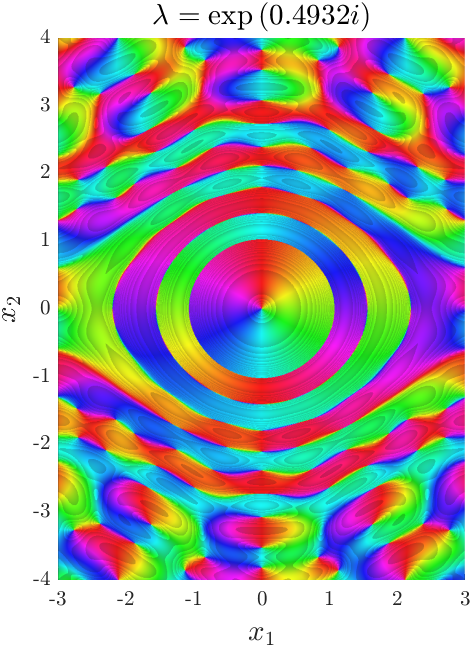
\includegraphics[width=0.25\linewidth]{../code/figures/pendulum/phase_portrait_4932.png}
        \hspace*{\fill}
        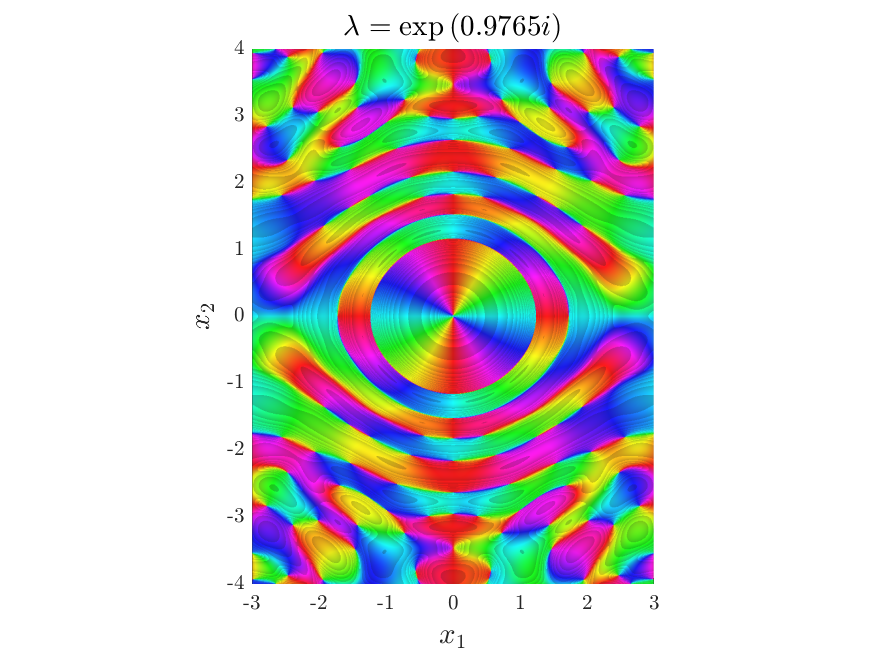
\includegraphics[width=0.25\linewidth]{../code/figures/pendulum/phase_portrait_9765.png}
        \hspace*{\fill}
        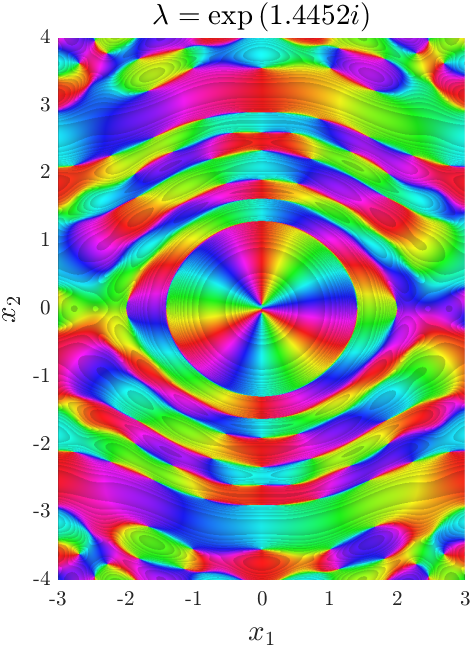
\includegraphics[width=0.25\linewidth]{../code/figures/pendulum/phase_portrait_14452.png}
        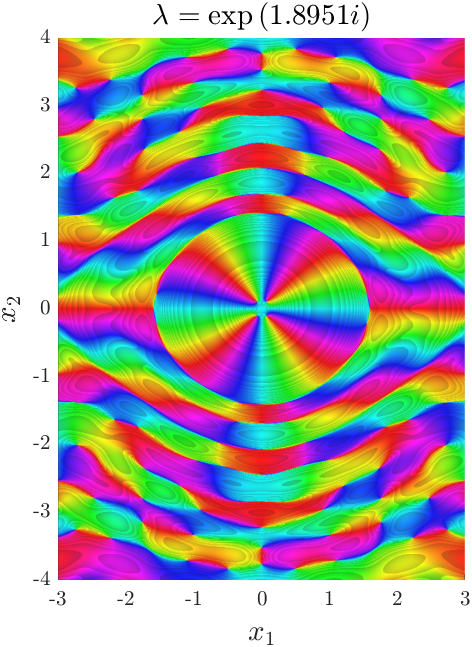
\includegraphics[width=0.25\linewidth]{../code/figures/pendulum/phase_portrait_18951.png}
        \hspace*{\fill}}
        \caption{Phase portraits of the approximate eigenfunctions of the nonlinear pendulum, where the color illustrates the complex argument of the eigenfunction. Lines of constant modulus are plotted as shadowed steps.}
        \label{pendulum_phase_portraits}
\end{figure}


\chapter{A kernel-based approach for high dimensional data}
\label{chapter_kedmd}
Until now, we supposed that the number of snapshots was large compared to the size of the dictionary, which also controls the number of eigenpairs approximated. However, when dealing with high dimensional data, we are usually in the opposite regime, where $K \gg M$. Indeed, as the dimension of the state space increases, the number of functions needed to have a rich enough dictionary overgrows. This blowup of the size $K$ of the dictionary occurs frequently in data-driven and Machine Learning related applications \cite{budisic_applied_2012, rowley_spectral_2009, schmid_dynamic_2010}, and it can be regarded as a facet of the so-called \emph{curse of dimensionality} \cite{bishop_pattern_2006}.  In this final chapter, we present Kernelized EDMD (K-EDMD), an algorithm that uses the kernel trick for a more efficient computation of the EDMD approximations. Unfortunately, having a dictionary size larger than the number of quadrature points makes ResDMD non applicable. This can be solved by using the two-steps procedure presented in \Cref{section_kresdmd}. Finally, we apply the previously mentioned two-steps procedure to the Gauss iterated map problem in order to obtain approximations of the Koopman eigenvalues without the need of a hand-crafted dictionary.

\section{Kernelized EDMD (K-EDMD)}
The EDMD algorithm necessitates the computation of the matrices $(\Psi_0^*\vb*{W}\Psi_0)$ and $(\Psi_0^*\vb*{W}\Psi_1)$, which requires $\mathcal{O}(MK^2)$ flops, and solving an eigenvalue problem associated to the matrix $\vb*{K}\in\C^{K\times K}$, which costs $\mathcal{O}(K^3)$ flops. For large values of $K$, such computations are impractical. \emph{Kernelized EDMD} (K-EDMD) \cite{williams_kernel-based_2015} uses the kernel trick \cite{bishop_pattern_2006} to efficiently compute a matrix $\hat{\vb*{K}}\in\C^{M\times M}$ that has the same non-zero eigenvalues as $\vb*{K}$. The computation of such a matrix relies on the following proposition.

\begin{prop}[\cite{colbrook_rigorous_2021}]
\label{prop_kedmd}
Let $\sqrt{\vb*{W}}\Psi_0 = \vb*{Q}\vb*{\Sigma}\vb*{Z}^*$ be a SVD, where $\vb*{\Sigma}\in\C^{M\times M}$ and let us define
\begin{equation}
    \label{kedmd_matrix}
    \hat{\vb*{K}} = (\vb*{\Sigma}^{\dagger}\vb*{Q}^*)(\sqrt{\vb*{W}}\Psi_1\Psi_0\sqrt{\vb*{W}})(\vb*{Q}\Sigma^{\dagger})\in\C^{M \times M}.
\end{equation}
Then $(\lambda,\,\vb{v})$ with $\lambda\neq 0$ is an eigenpair of $\hat{\vb*{K}}$ if and only if $(\lambda,\,\vb*{Z}\vb{v})$ is an eigenpair of $\vb*{K}$, where $\vb*{K}$ is defined in \eqref{discretized_problem_solution}.
\end{prop}
\begin{proof}
Let us recall that the matrix $\vb*{K}$ is defined in \eqref{discretized_problem_solution} as $\vb*{K} = (\Psi_0^*\vb*{W}\Psi_0)^{\dagger}(\Psi_0^*\vb*{W}\Psi_1)$. For a generic matrix $\vb*{A}$, the following two properties of the Moore-Penrose inverse hold: $(\vb*{A}^*\vb*{A})^{\dagger}\vb*{A}^* = \vb*{A}^{\dagger}$ and $\range(\vb*{A}^{\dagger}) = \range(\vb*{A}^*)$, where $\range(\vb*{A})$ denotes the Span of the columns (or range) of $\vb*{A}$. Applying these two properties to the matrix $\vb*{A} = \sqrt{\vb*{W}}\Psi_0$ it follows: 
\begin{equation*}
    \begin{split}
        &\vb*{K} = (\Psi_0^*\vb*{W}\Psi_0)^{\dagger}(\Psi_0^*\vb*{W}\Psi_1) = (\sqrt{\vb*{W}}\Psi_0)^{\dagger} \sqrt{\vb*{W}}\Psi_1 \\
        &\range(\vb*{K}) \subseteq \range((\sqrt{\vb*{W}}\Psi_0)^{\dagger}) = \range(\sqrt{\vb*{W}}\Psi_0)^*)
    \end{split}
\end{equation*}
Hence any eigenvector $\vb{v}$ such that $\vb*{K}\vb{v} = \lambda \vb{v}$ with $\lambda \neq 0$ can be written as $\vb{v} = (\sqrt{\vb*{W}}\Psi_0)^*\tilde{\vb{v}} = \vb*{Z}\vb*{\Sigma}\vb*{Q}^*\tilde{\vb{v}} = \vb*{Z}\hat{\vb{v}}$ for some $\hat{\vb{v}}$. Thus:
\begin{equation*}
    \lambda \vb*{Z}\hat{\vb{v}} = \vb*{K}\vb*{Z}\hat{\vb{v}} = (\sqrt{\vb*{W}}\Psi_0)^{\dagger} \sqrt{\vb*{W}}\Psi_1 \vb*{Z}\hat{\vb{v}} = \vb*{Z}\left[(\vb*{\Sigma}^{\dagger}\vb*{Q}^*)(\sqrt{\vb*{W}}\Psi_1\Psi_0\sqrt{\vb*{W}})(\vb*{Q}\Sigma^{\dagger})\right] \hat{\vb{v}}
\end{equation*}
and multiplying by $\vb*{Z}^*$ on the right we obtain that if $(\lambda,\,\vb{v})$ is an eigenpair of $\vb*{K}$ with $\lambda\neq 0$, then $(\lambda,\,\hat{\vb{v}} = \vb*{Z}^*\vb{v})$ is an eigenpair of $\hat{\vb*{K}}$. 

Vice versa, if $(\lambda,\,\vb{v})$ is an eigenpair of $\hat{\vb*{K}}$, then:
\begin{equation*}
    \vb*{K}\vb*{Z}\vb{v} = \vb*{Z}\hat{\vb*{K}}\vb{v} = \lambda\vb*{Z}\vb{v}
\end{equation*}
i.e. $(\lambda,\,\vb*{Z}\vb{v})$ is an eigenpair of $\vb*{K}$.
\end{proof}

Now observe that to build the matrix $\hat{\vb*{K}}$ we just need to compute inner products of evaluation of our dictionary. The matrices $\vb*{Q}$ and $\vb*{\Sigma}$ can be obtained from the eigenvalue decomposition of $\sqrt{\vb*{W}}\Psi_0\Psi_0^*\sqrt{\vb*{W}} = \vb*{Q}\vb*{\Sigma}^2\vb*{Q}^*$, and both $(\sqrt{\vb*{W}}\Psi_0\Psi_0^*\sqrt{\vb*{W}})$ and $(\sqrt{\vb*{W}}\Psi_1\Psi_0^*\sqrt{\vb*{W}})$ can be computed using inner products only. Indeed, recalling that $\Psi(\vb{x})$ is a row vector:
\begin{equation}
    \label{kernel_matrices}
    \begin{split}
        (\sqrt{\vb*{W}}\Psi_0\Psi_0^*\sqrt{\vb*{W}})_{ij} &= \sqrt{w_i} \Psi(\vb{x}_0^{(i)}) \Psi(\vb{x}_0^{(j)})^* \sqrt{w_j}\\
        (\sqrt{\vb*{W}}\Psi_1\Psi_0^*\sqrt{\vb*{W}})_{ij} &= \sqrt{w_i} \Psi(\vb{x}_1^{(i)}) \Psi(\vb{x}_0^{(j)})^* \sqrt{w_j}.
    \end{split}
\end{equation}
The kernel trick \cite{bishop_pattern_2006} is a common technique used to compute these inner products implicitly. Instead of first evaluating the dictionary $\Psi(\vb{x})$ and then computing the inner product, that would require $\mathcal{O}(K)$ operations, we compute $\kappa(\vb{x}, \vb{y}) = \Psi(\vb{x})\Psi(\vb{y})^*$ for a suitably defined kernel $\kappa$. It is crucial that the kernel $\kappa$ does not compute the inner product directly, but it does so implicitly in $\mathcal{O}(d)$ operations, where $d$ is the data dimension. Thus the matrices $(\sqrt{\vb*{W}}\Psi_0\Psi_0^*\sqrt{\vb*{W}})$ and $(\sqrt{\vb*{W}}\Psi_1\Psi_0^*\sqrt{\vb*{W}})$ can be calculated in $\mathcal{O}(dM^2)$ operations, without suffering from the large size of the dictionary. The total complexity of computing $\hat{\vb*{K}}$ and solving the associated eigenvalue problem is $\mathcal{O}(d M^2 + M^3)$, significantly lower than the $\mathcal{O}(M K^2+K^3)$ cost of applying EDMD directly. 

\subsection{Computing the Koopman eigenvalues, eigenfunctions and modes}
Once we have computed the matrix $\hat{\vb*{K}}$ and its eigendecomposition, we still need to understand how to retrieve from it an approximation of the Koopman eigenvalues, eigenfunctions and modes. The eigenvalues of $\hat{\vb*{K}}$ can be directly used as approximation of the Koopman eigenvalues. Let $\hat{\bm{\Xi}} = \left[\hat{\bm{\xi}}_1,\dots,\hat{\bm{\xi}}_M\right]$ be the matrix of the eigenvectors of $\hat{\vb*{K}}$, the vector of approximate Koopman eigenfunctions $\Phi(\vb{x}) = \left[\phi_1(\vb{x}), \dots, \phi_M(\vb{x})\right]$ can be written as $\Phi = \Psi\vb*{Z}\hat{\bm{\Xi}} = \Psi (\Psi_0^*\sqrt{\vb*{W}})(\vb*{Q}\Sigma^{\dagger}) \hat{\bm{\Xi}}$. All we have done so far would not be useful if we suffered from the size of the dictionary when approximating the Koopman eigenfunctions. Fortunately, it is possible to express them using kernels only. Indeed:
\begin{equation}
    \label{kernel_eigenfunctions}
    \begin{split}
        \phi_k(\vb{x}) &= \Psi(\vb{x}) (\Psi_0^*\sqrt{\vb*{W}})(\vb*{Q}\Sigma^{\dagger}) \hat{\bm{\xi}}_k =\\
        &= \left[\sqrt{w_1} \kappa(\vb{x}, \vb{x}_0^{(1)}), \dots, \sqrt{w_M} \kappa(\vb{x}, \vb{x}_0^{(M)})\right](\vb*{Q}\Sigma^{\dagger}) \hat{\bm{\xi}}_k
    \end{split}
\end{equation}
so that the size $K$ of the dictionary does not enter any of the computations.

To compute the Koopman modes of the full state observable, we consider equation \eqref{koopman_modes} and we evaluate it at each of the data points using the approximate eigenfunctions we just obtained. When evaluated at $\vb{x}_0^{(i)}$ the equation reads:
\begin{equation}
    \label{kedmd_modes_pointwise}
    \vb{x}_0^{(i)} = \sum_{j = 1}^M \phi_j(\vb{x}_0^{(i)})\hat{\vb{v}}_{j} + \vb{r}_i
\end{equation}
where $\{\hat{\vb{v}}_{j}\}_{j=1}^M$ are the Koopman modes that we want to retrieve and $\vb{r}_i$ is a residual that must be minimized. If we introduce the matrices
\begin{equation}
    \begin{split}
    \vb*{X} = 
    \begin{bmatrix}
    (\vb{x}_0^{(1)})^T \\
    \vdots \\
    (\vb{x}_0^{(M)})^T
    \end{bmatrix}&,
    \\ 
    \Phi_0 = 
    \begin{bmatrix}
    \Phi(\vb{x}_0^{(1)}) \\
    \vdots \\
    \Phi(\vb{x}_0^{(M)})
    \end{bmatrix}&
    = \Psi_0 \vb*{Z}\hat{\bm{\Xi}} = \Psi_0 (\Psi_0^*\sqrt{\vb*{W}})(\vb*{Q}\Sigma^{\dagger}) \hat{\bm{\Xi}} =\\
    & = \sqrt{\vb*{W}^{-1}} \vb*{Q}\vb*{\Sigma}^2\vb*{Q}^*\vb*{Q}\Sigma^{\dagger}\hat{\bm{\Xi}} = \sqrt{\vb*{W}^{-1}} \vb*{Q}\Sigma\hat{\bm{\Xi}}
    \end{split}
\end{equation}
i.e. the data-points matrix and the matrix of the eigenfunctions values at those points, \eqref{kedmd_modes_pointwise} can be rewritten as
\begin{equation}
    \label{kedmd_modes_matrix}
    \vb*{X} = \Psi_0 \hat{\vb*{V}} + \vb*{R}.
\end{equation}
The solution to the least squares problem is 
\begin{equation}
    \hat{\vb*{V}} =  
    \begin{bmatrix}
    \hat{\vb{v}}_1^T \\
    \vdots \\
    \hat{\vb{v}}_M^T
    \end{bmatrix}
    = \Psi_0^{\dagger} \vb*{X} = \hat{\bm{\Xi}}^{-1} \Sigma^{\dagger} \vb*{Q}^* \sqrt{\vb*{W}} \vb*{X}.
\end{equation}
Hence the approximation of the $j$-th Koopman mode is 
\begin{equation}
    \label{kedmd_modes}
    \hat{\vb{v}}_j = (\hat{\vb{u}}_j^* \Sigma^{\dagger} \vb*{Q}^* \sqrt{\vb*{W}} \vb*{X})^T
\end{equation}
where $\hat{\vb{u}}_j$ is a left eigenvector of $\hat{\vb*{K}}$ appropriately scaled so that $\hat{\vb{u}}_j^*\hat{\bm{\xi}}_i = \delta_{ij}$.

\subsection{The choice of the kernel}
Even if in the previous discussion we supposed that, given a dictionary $\Psi(\vb{x})$, there exists a kernel $\kappa$ that computes $\kappa(\vb{x}, \vb{y}) = \Psi(\vb{x})\Psi(\vb{y})^*$ implicitly, in effect it is usually the choice of $\kappa$ that defines the dictionary. One of the most simple kernels is the polynomial kernel $\kappa(\vb{x}, \vb{y}) = (1 + \vb{x}^*\vb{y})^{n}$, which is equivalent to a dictionary that can represent all polynomials up to degree $n$. Increasing $n$ the implicitly defined dictionary becomes larger, at the cost of a worst conditioning of the resulting matrices. For this reason, taking inspiration from Machine Learning techniques, other kernels could be considered, such as the widely used radial basis function kernel (RBF kernel), $\kappa(\vb{x}, \vb{y}) = \exp(-\norm{\vb{x}-\vb{y}}^2 / \sigma^2)$.

\begin{algorithm}[h]
\caption{\textbf{: Kernelized EDMD (K-EDMD)}}
\label{alg_kedmd}
\textbf{Input:} Snapshot pairs of the system state, $\{(\vb{x}_0^{(m)}, \vb{x}_1^{(m)})\}_{m = 1}^M$, quadrature weights $\{w_m\}_{m = 1}^M$, kernel $\kappa = \kappa(\cdot\,,\,\cdot)$.
\begin{algorithmic}[1]
\State  Compute the matrices $\hat{\vb*{G}} = \sqrt{\vb*{W}}\Psi_0\Psi_0^*\sqrt{\vb*{W}}$ and  $\hat{\vb*{A}} = \sqrt{\vb*{W}}\Psi_1\Psi_0^*\sqrt{\vb*{W}}$, exploiting that $\hat{\vb*{G}}_{ij} = \sqrt{w_i} \kappa(\vb{x}_0^{(i)},\, \vb{x}_0^{(j)}) \sqrt{w_j}$ and
$\hat{\vb*{A}}_{ij} = \sqrt{w_i} \kappa(\vb{x}_1^{(i)},\, \vb{x}_0^{(j)}) \sqrt{w_j}$.
\State Compute the eigenvalue decomposition of $\hat{\vb*{G}} = \vb*{Q}\vb*{\Sigma}^2\vb*{Q}^*$.
\State Compute $\hat{\vb*{K}} = (\vb*{\Sigma}^{\dagger}\vb*{Q}^*)\hat{\vb*{A}} (\vb*{Q}\Sigma^{\dagger})$.
\State Solve the eigenvalue problem of $\hat{\vb*{K}}\hat{\bm{\xi}} = \lambda \hat{\bm{\xi}}$.
\State Obtain the eigenfunctions as $\phi_k(\vb{x}) = \left[\sqrt{w_1} \kappa(\vb{x}, \vb{x}_0^{(1)}), \dots, \sqrt{w_M} \kappa(\vb{x}, \vb{x}_0^{(M)})\right](\vb*{Q}\Sigma^{\dagger}) \hat{\bm{\xi}}_k$.
\If{want to compute eigenmodes}
    \State Compute the left eigenvectors $\vb{u}_j$ of $\hat{\vb*{K}}$ appropriately scaled so that $\hat{\vb{u}}_j^*\hat{\bm{\xi}}_i = \delta_{ij}$.
    \State Compute $\hat{\vb*{B}} = \Sigma^{\dagger} \vb*{Q}^* \sqrt{\vb*{W}} \vb*{X}$.
    \State Obtain the modes as $\hat{\vb{v}}_j = (\hat{\vb{u}}_j^* \hat{\vb*{B}})^T$.
\EndIf
\end{algorithmic}
\textbf{Output:} Approximation of the eigenvalues ($\lambda_j$), eigenfunctions ($\phi_j$) and, possibly, eigemodes ($\vb{v}_j$).
\end{algorithm}

\section{Kernelized ResDMD (K-ResDMD)}
\label{section_kresdmd}
At this point, it is a natural question how one could extend ResDMD with a kernelized approach. Unfortunately, applying \Cref{alg_resdmd} with K-EDMD instead of EDMD makes the approximate residual always vanish (see \cite{colbrook_rigorous_2021}, Proposition 6.2). Basically, since the size of our function space is larger than the number of snapshots, we can "interpolate", and we are actually overfitting our dataset. Similarly to what is done when training and testing a Machine Learning model, to have a reliable estimate of the residual for approximate eigenpairs, we need to compute it using quadrature points that have not been used at the "interpolation stage" and that, at least ideally, are independent of the ones previously employed. This idea leads to the following multi-step approach:
\begin{enumerate}
    \item Split the snapshot data into two (ideally independent) sets $\{(\vb{x}_0^{(j)},\,\vb{x}_1^{(j)})\}_{j=1}^{M'}$ and  $\{(\vb{y}_0^{(j)},\,\vb{y}_1^{(j)})\}_{j=1}^{M''}$, with $M'' \geq M'$.
    \item Apply K-EDMD to the first data set $\{(\vb{x}_0^{(j)},\,\vb{x}_1^{(j)})\}_{j=1}^{M'}$, and compute a dictionary that Spans the function space generate by the approximations of dominant $K' < M'$ eigenfunctions (see \Cref{alg_kresdmd} for the details). Let us denote this dictionary as $\Psi(x) = \left[\psi_1(\vb{x}), \dots, \psi_{K'}(\vb{x})\right]$.
    \item Apply \Cref{alg_resdmd} or \Cref{alg_pseudospectrum} with snapshot data $\{(\vb{y}_0^{(j)},\,\vb{y}_1^{(j)})\}_{j=1}^{M''}$ and dictionary $\Psi(x)$.
\end{enumerate}
As summarized in \Cref{alg_kresdmd} in the first stage, we reduce the size of the dictionary implicitly defined by the kernel to $K'$, hoping to obtain a good dictionary that already captures the essential dynamics. Then this dictionary is used as a basis for the ResDMD algorithm, which computes reliable approximations of the eigenpairs of the Koopman operator. This also provides an a posteriori check of the quality of the dictionary obtained in the first stage.

\begin{algorithm}[h]
\caption{\textbf{: Kernelized ResDMD (K-ResDMD)}}
\label{alg_kresdmd}
\textbf{Input:} Snapshot pairs of the system state, $\{(\vb{x}_0^{(m)}, \vb{x}_1^{(m)})\}_{m = 1}^M$, quadrature weights $\{w_m\}_{m = 1}^M$, kernel $\kappa = \kappa(\cdot\,,\,\cdot)$, hyperparameters $M', \,M'', \,K'$.
\begin{algorithmic}[1]
\State  Split the snapshot data into $\{(\vb{x}_0^{(j)},\,\vb{x}_1^{(j)})\}_{j=1}^{M'}$ and  $\{(\vb{y}_0^{(j)},\,\vb{y}_1^{(j)})\}_{j=1}^{M''}$, with $M = M' + M''$ and $M'' \geq M' > K'$.
\State Apply K-EDMD (\Cref{alg_kedmd}) with snapshot pairs $\{(\vb{x}_0^{(j)},\,\vb{x}_1^{(j)})\}_{j=1}^{M'}$: compute the dominant $K' < M'$ eigenvectors of $\hat{\vb*{K}}$ and stack them into $\hat{\bm{\Xi}} = \left[\hat{\bm{\xi}}_1, \dots, \hat{\bm{\xi}}_{K'}\right]$. 
\State Orthogonalize the colums of $\hat{\bm{\Xi}}$ to $\vb*{P} = [\vb{p}_1, \dots, \vb{p}_{K'}]$.
\State Apply \Cref{alg_resdmd} or \Cref{alg_pseudospectrum} with snapshot data $\{(\vb{y}_0^{(j)},\,\vb{y}_1^{(j)})\}_{j=1}^{M''}$ and dictionary $\{\psi_j\}_{j = 1}^{K'}$ defined by
\begin{equation*}
    \psi_j(\vb{x}) = \left[\sqrt{w_1} \kappa(\vb{x}, \vb{x}_0^{(1)}), \dots, \sqrt{w_M} \kappa(\vb{x}, \vb{x}_0^{(M')})\right](\vb*{Q}\Sigma^{\dagger})\, \vb{p}_j
\end{equation*}
\end{algorithmic}
\textbf{Output:} According to the algorithm chosen in the final step.
\end{algorithm}

\section{A numerical example: a data-driven dictionary for the Gauss iterated map}
The two-steps procedure just presented is applied in \cite{colbrook_rigorous_2021} to deal with high dimensional data. However, it might also be used for low dimensional data as a way to apply EDMD and ResDMD to different problems without the need of manually designing a different dictionary according to the properties of each problem. In this section, we applied it to the Gauss iterated map problem previously introduced in \Cref{sect_gauss_iterated_map}. 

To experimentally show the effects of having a dictionary of observables with a size larger or equal than the the number of quadrature points, we first considered the ResDMD algorithm and the K-EDMD algorithm applied with the same dictionary of observables. To do so, we considered as a dictionary $\Phi(x)$ for the ResDMD algorithm the first $K=40$ Legendre polynomials transferred to the interval $\Omega = [-1,0]$ and as a kernel for the K-EDMD algorithm the kernel defined by $\Phi$, i.e. $\kappa(x,y) = \Phi(x)\Phi(y)^\star$. As snapshot pairs we considered $\{(\vb{x}_0^{(m)}, \vb{x}_1^{(m)})\}_{m = 1}^M$ with $M=K=40$, where $\{(\vb{x}_0^{(m)}\}_{m = 1}^M$ are the Gauss-Legendre quadrature nodes transplanted to $\Omega$ and $\vb{x}_1^{(m)} = F(\vb{x}_0^{(m)})$. For the ResDMD algorithm, we discard approximate eigenvalues with an estimated residual lower than $\varepsilon = 0.1$. \Cref{fig_kedmd_vs_edmd} shows the output of the ResDMD and K-EDMD algorithms. As expected from \Cref{prop_kedmd} the output of the two algorithms coincides. However, since the number of snapshot pairs $M$ is equal to the size $K$ of the dictionary, the ResDMD algorithm does not discard any of the approximated eigenvalues in output of the EDMD algorithm.  
\begin{figure}[h]
\centering
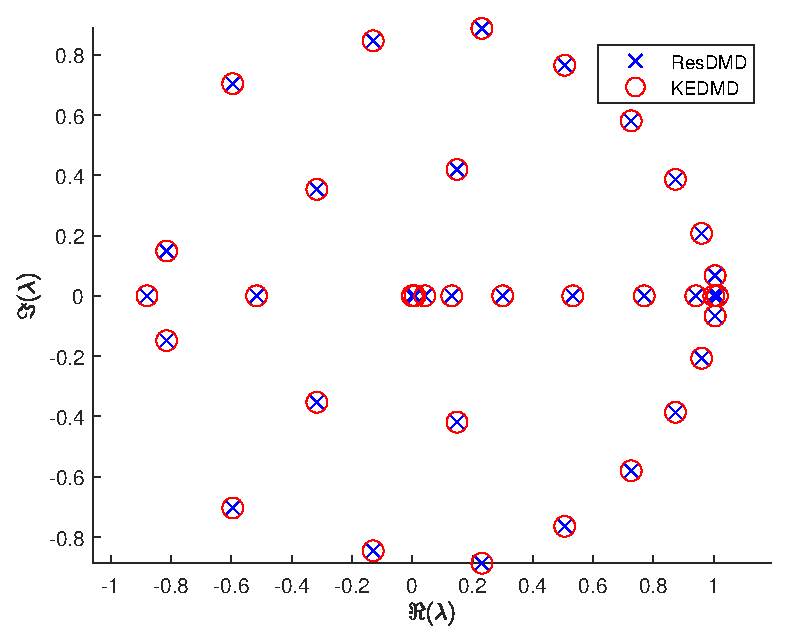
\includegraphics[width=0.55\linewidth]{../code/figures/gauss_map/kernelized/KEDMD_Gauss-Legendre.eps}
\caption{Output of the ResDMD ad K-EDMD algorithm for the Gauss iterated map problem, when using a number of snapshots pairs $M = 40$ equal to the size $K$ of the dictionary, and the kernel defined by the dictionary. The firs $K$ Legendre polynomials are used as a dictionary and the Gauss-Legendre quadrature points as initial snapshots.}
\label{fig_kedmd_vs_edmd}
\end{figure}

Finally, to analyse the effectiveness of the procedure for extracting a dictionary from a general-purpose kernel, we applied the two-stages Kernelized ResDMD algorithm with a RBF kernel. Let us observe that the RBF kernel can be seen as the inner product of an infinite polynomial dictionary, hence we do not have any constraint on the number of snapshot datapoints. As snapshot data for the first stage, we considered $M' = 1000$ Montecarlo quadrature nodes and we extracted the $K' = 40$ dominant eigenpairs using the K-EDMD algorithm. In the second stage, we applied the ResDMD algorithm using the dictionary in output of the K-EDMD algorithm and $M''=1000$ Gauss-Legendre quadrature points as snapshot data. The tolerance employed in K-ResDMD was $\varepsilon = 0.01$. As suggested in \cite{colbrook_rigorous_2021}, we also employed the following common practices:
\begin{itemize}
    \item the constant $\sigma$ of the RBF kernel $\kappa(\vb{x}, \vb{y}) = \exp(-\norm{\vb{x}-\vb{y}}^2 / \sigma^2)$ was set as the average $\ell^2$-norm of the snapshot data after it is shifted to have mean zero.
    \item the gramian matrices of the first stage $\hat{\vb*{G}} = \sqrt{\vb*{W}}\Psi_0\Psi_0^*\sqrt{\vb*{W}}$ and  $\hat{\vb*{A}} = \sqrt{\vb*{W}}\Psi_1\Psi_0^*\sqrt{\vb*{W}}$ are both ill conditioned, with a conditioning number of the order $10^{20}$ and a numerical rank between $40$ and $50$ (their size is $M'=1000$). Therefore, we added regularization in the form $\hat{\vb*{G}} = \hat{\vb*{G}} + \eta \lVert\hat{\vb*{G}}\rVert_F \vb*{I}$ where $\eta = 10^{-16}$. 
\end{itemize}
\Cref{fig_2steps_kedmd} shows the results of the above described procedure. The pseudospectral contour lines computed in \Cref{sect_gauss_iterated_map} are plotted as a reference to evaluate the quality of the approximated eigenvalues. It can be observed that the approximated eigenvalues returned by the K-ResDMD via the two-step extraction procedure are very similar to the ones shown in \Cref{gauss_pseudospectrum_convergence}, obtained using the ResDMD, and they all lie inside the $0.01$-pseudospectrum approximation previously computed. However, the eigenvalues shown in \Cref{fig_2steps_kedmd} did not require a hand-crafted dictionary in input to the algorithm, but employed the general-purpose RBF kernel with the scaling factor $\sigma$ determined using the data. 

\begin{figure}[h]
\centering
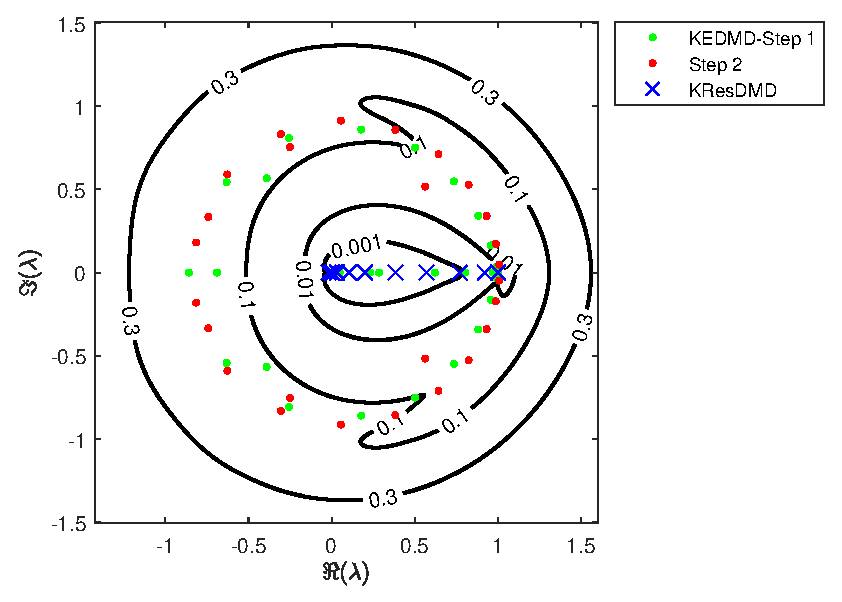
\includegraphics[width=0.70\linewidth]{../code/figures/gauss_map/kernelized/KEDMD_2step_rbf_Montecarlo.eps}
\caption{Eigenvalues approximation for the Gauss iterated map problem, obtained using the two-step procedure described in \Cref{alg_kresdmd}. Green dots show the $K'=40$ dominant eigenvalues computed in the first step. Eigenvalues returned in the second steps are represented as red dots and blue crosses, where blue crosses show the eigenvalues retained by K-ResDMD with tolerance $\epsilon = 0.01$. The pseudospectral contour lines computed in \Cref{sect_gauss_iterated_map} are also plotted as a reference.}
\label{fig_2steps_kedmd}
\end{figure}


\chapter{Conclusions}
Starting from the article \cite{colbrook_rigorous_2021} by Colbrook and Townsend, we analysed spectral properties of the Koopman Operator and discussed methods to numerically compute spectral approximations. Dynamic Mode Decomposition was presented, with a particular focus on the case of linear dynamical systems, where DMD is mathematically equivalent to the Arnoldi algorithm but less stable from a numerical point of view. For nonlinear dynamics, the EDMD algorithm was proposed, and its variant ResDMD was used to both deal with the problem of spectral pollution and approximate the pseudospectrum of the Koopman Operator. Furthermore, a proposition linking the pseudospectral approximation returned by ResDMD and the pseudospectrum of a particular matrix pencil was proven in this work. Two numerical examples from Section 4 of \cite{colbrook_rigorous_2021} were reproduced in details: the Gauss iterated map and the nonlinear pendulum. Finally, the kernelized approach proposed in \cite{colbrook_rigorous_2021} for high dimensional data was used to create a data-driven dictionary for the Gauss iterated map problem to show a possible way of avoiding the step of hand-crafting a problem-dependent dictionary for the EDMD and ResDMD algorithms.

%BIBLIOGRAPHY
\nocite{*}
\printbibliography

\end{document}

\end{document}